
\chapter{Applications of Multivariate Analysis in Metabolomics}

\section{Introduction}

\begin{doublespace}
This chapter details several varied applications of multivariate analysis
within the field of metabolomics, from the simplest examples of constructing
multivariate calibration models of \hnmr{} NMR spectral data for determination
of caffeine concentration in coffee, to more complex examples of multiblock
statistical modeling of joint \hnmr{} NMR and electrospray MS data. A final
note on the relationship between PCA scores-space class separations and OPLS-DA
model reliability is also presented to conclude the chapter.
\end{doublespace}

\section{\hnmr{} NMR Fingerprinting of Brewed Coffees}

\begin{doublespace}
To provide an initial illustration of the capabilities of the MVAPACK software
suite \cite{worley:acscb2014}, four roasts of brewed coffee were purchased from
a local coffee shop. In this study, \hnmr{} NMR and UV/Vis absorbance spectra
were collected in order to construct a multivariate calibration of \hnmr{} NMR
spectral information against caffeine concentration.
\end{doublespace}

\subsection{Materials and Methods}

\subsubsection{Coffee Sample Preparation}

\begin{doublespace}
Four freshly brewed roasts of coffee (Light, Dark, Medium Regular and Medium
Decaffeinated) were purchased from a local coffee shop. From each roast,
sixteen 1.2 mL samples were drawn while the coffee was still hot and stored
at $-80^\circ$C for 24 hours. The samples were then lyophilized at
$-50^\circ$C and 0.1 mBar for 24 hours and subsequently redissolved in 1.0 mL
of 99.8\% D$_2$O (Isotec, St. Louis, MO) without pH adjustment. Following
redissolution, the samples were centrifuged at 12,000 RPM and $25^\circ$C
for 5 minutes and 800 $\mu$L of the supernatant was collected into NMR tubes.
The samples were stored in their NMR tubes at $4^\circ$C for 36 hours prior
to data collection.
\end{doublespace}

\subsubsection{Caffeine Extraction}

\begin{doublespace}
Measurement of the caffeine concentration in each coffee roast was performed
based on previously outlined procedures \cite{belay:food2008}. Triplicate
standards of caffeine were made by dissolving 2.9 mg of caffeine
(Sigma-Aldrich, St. Louis, MO) into 100.0 mL of 99.5\% CH$_2$Cl$_2$
(Sigma-Aldrich, St. Louis, MO) for a final concentration of 149 $\mu$M.
From each purchased coffee roast, 25 mL of brewed coffee were combined with
25 mL of CH$_2$Cl$_2$ in a separatory funnel in a two-step liquid-liquid
extraction. Extracted caffeine in CH$_2$Cl$_2$ was diluted 20-fold into 1.0
mL and subjected to UV/Vis absorption spectroscopy for caffeine quantitation.
\end{doublespace}

\begin{figure}[ht!]
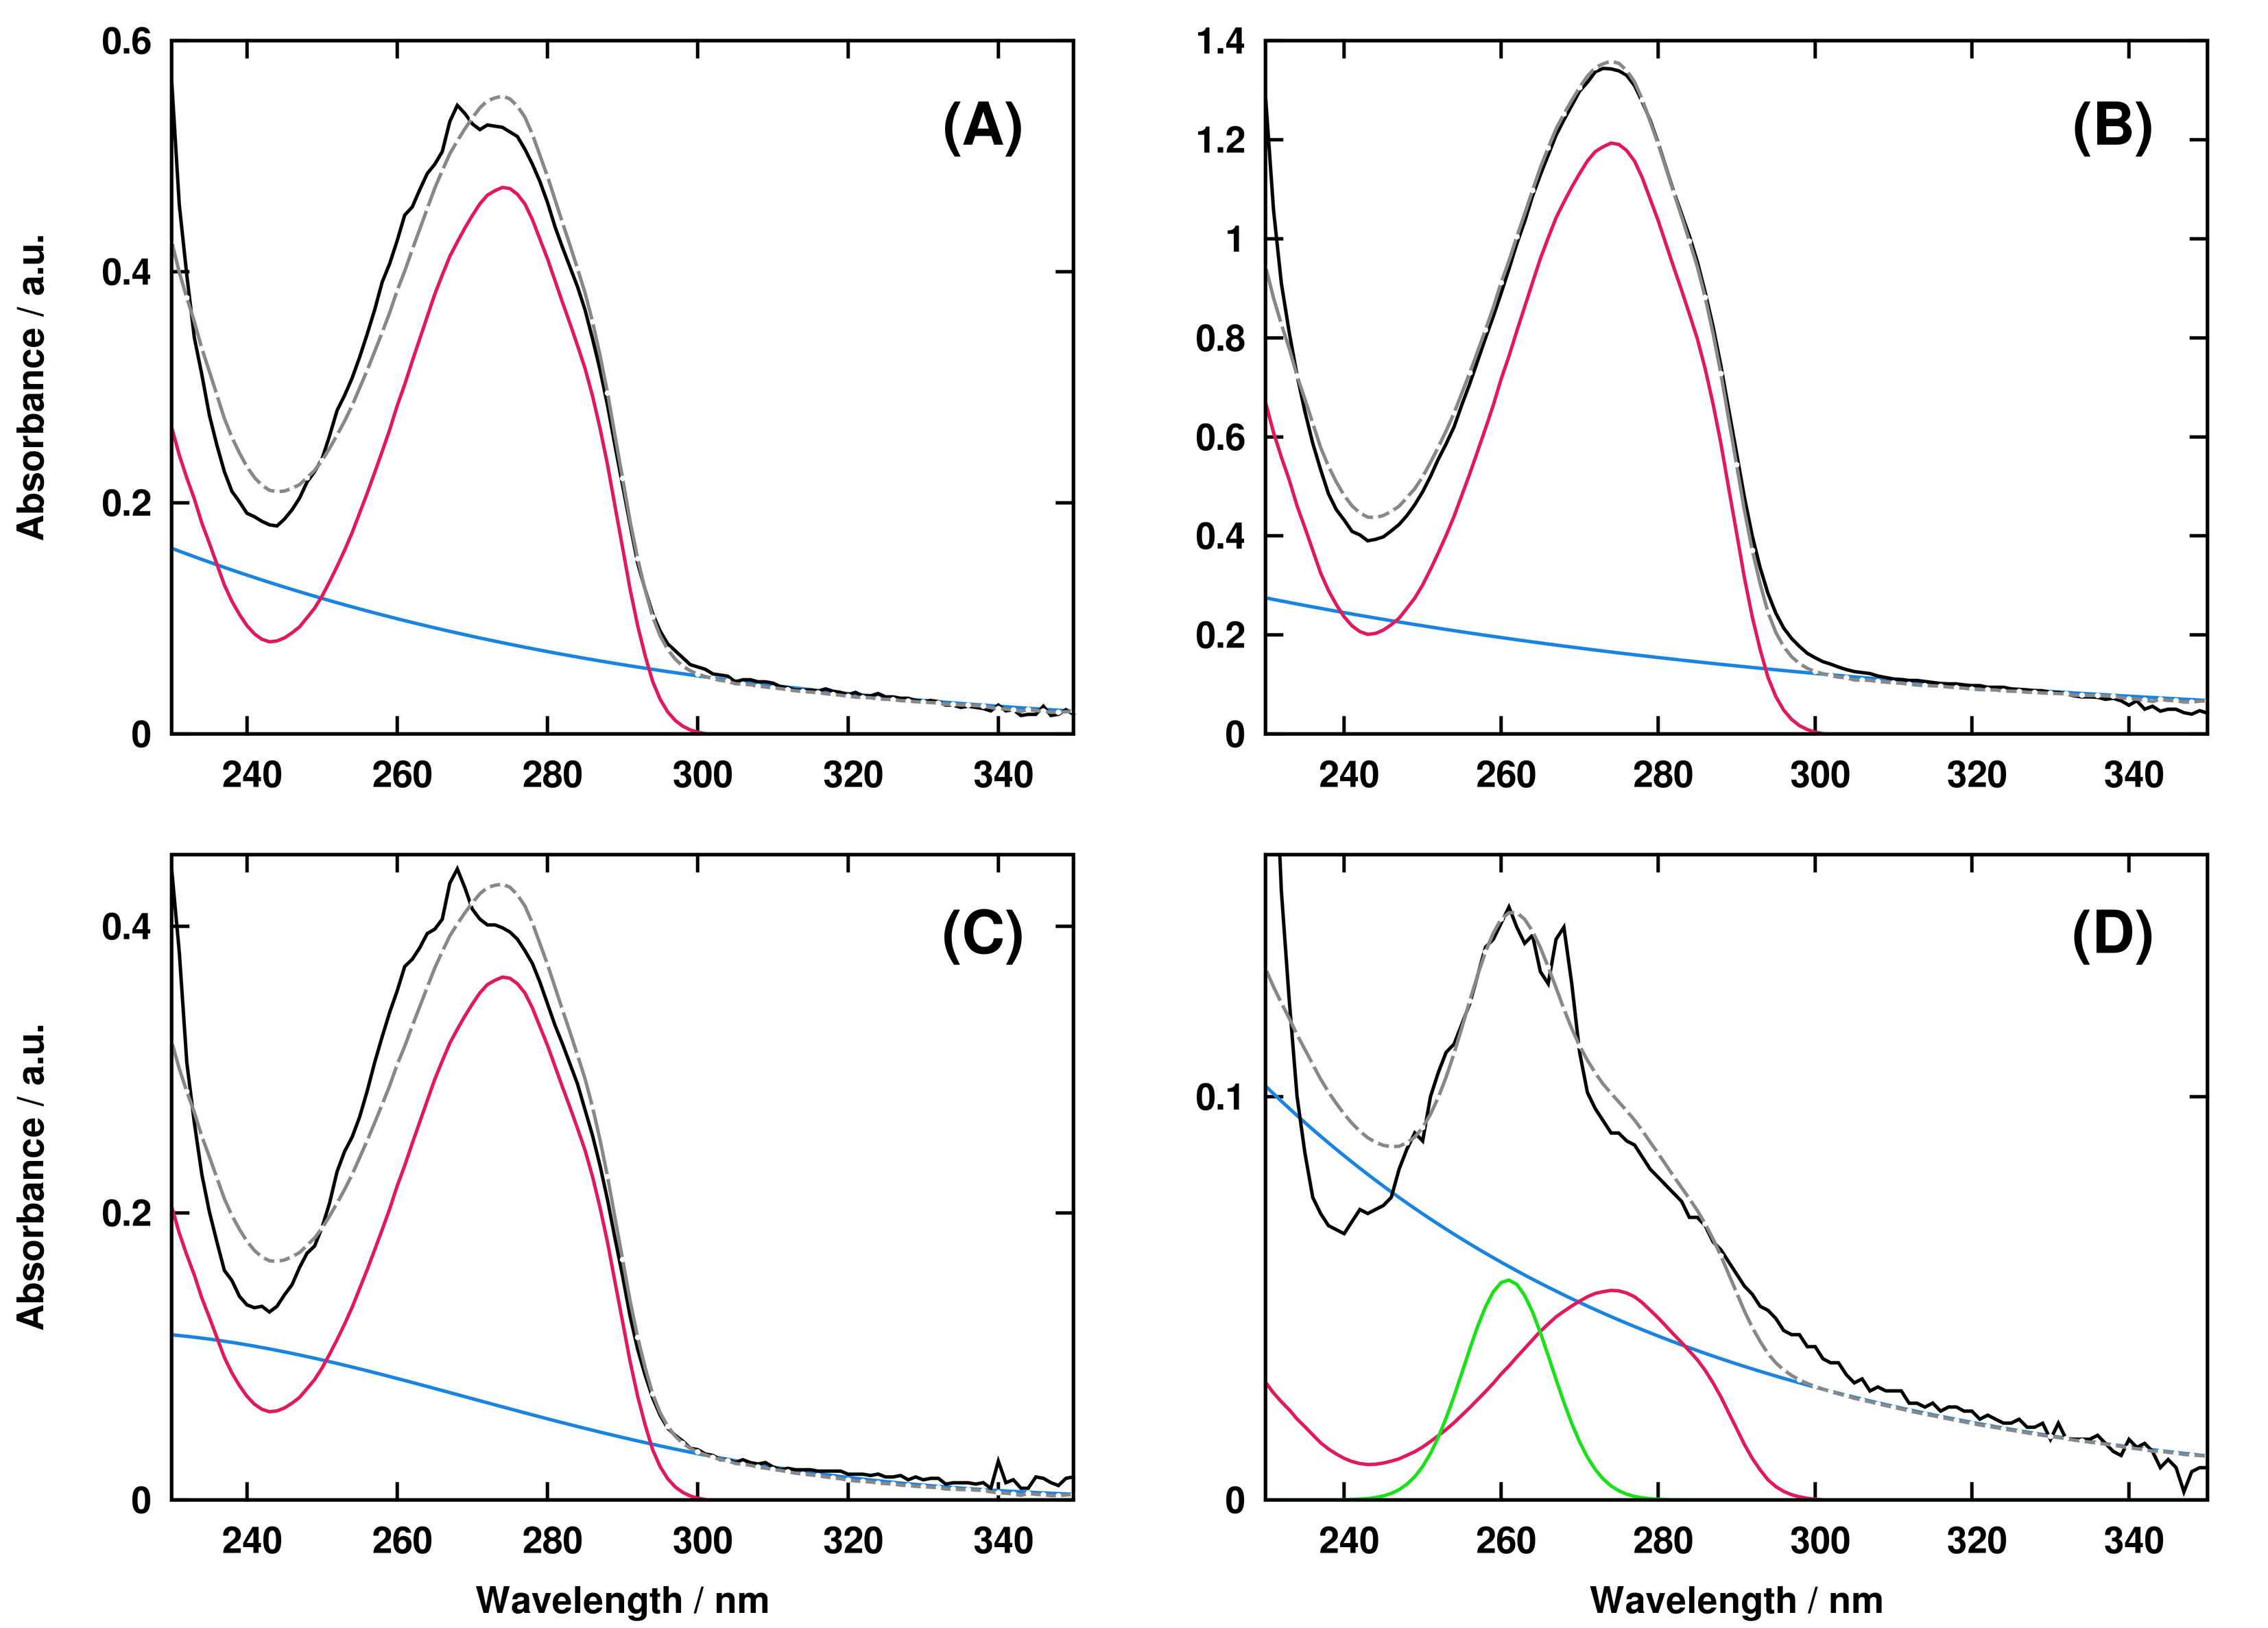
\includegraphics[width=6in]{figs/apps/01-uvfit.png}
\caption
      [UV/Vis Caffeine Quantitation Band-fitting Results.]{
  {\bf UV/Vis Caffeine Quantitation Band-fitting Results.}
  \\
  UV/Vis absorbance band-fitting results for caffeine concentration estimation
  of dark roast ({\bf A}), light roast ({\bf B}), regular medium roast
  ({\bf C}), and decaffeinated medium roast ({\bf D}). Black lines represent
  observed spectra, dashed grey lines represent fitted spctra, red lines
  represent fitted caffeine, and blue and green lines represent additional
  Gaussian bands required for fitting.
}
\label{figure.4.1}
\end{figure}

\subsubsection{UV/Vis Spectroscopy}

\begin{doublespace}
Absorption spectra of caffeine standards and extracts were collected on a
Shimadzu UV-2501PC with a 1.0 nm slit width and 1.0 cm quartz cuvettes. Spectra
were collected between the wavelengths of 500 nm and 230 nm.
\end{doublespace}

\subsubsection{NMR Spectroscopy}

\begin{doublespace}
All NMR experiments were collected on a Bruker Avance DRX 500 MHz spectrometer
equipped with a 5 mm inverse triple-resonance (\hnmr{}, \cnmr{}, \nnmr{})
cryoprobe with a $z$-axis gradient. A Bruker BACS-120 sample changer and
ICON-NMR software were used to automate NMR data collection. A standard 1D
\hnmr{} NMR spectrum using a SOGGY pulse sequence
\cite{hwang:jmr1995,nguyen:jmr2007} and a $T_2$-filtered 1D \hnmr{} NMR
spectrum using a $z$-filtered Carr-Purcell-Meiboom-Gill (CPMG) sequence
\cite{rastrelli:jacs2009} with an identical SOGGY water suppression element
were acquired for each sample. All experiments were performed at $20^\circ$C
with 128 scans, 32 dummy scans, a carrier frequency offset of 2,351 Hz, a
6,009 Hz spectral width, and a 1.0 s inter-scan delay. For $T_2$ filtered
spectra, 20 repetitions of a CPMG-$z$ element having a delay ($\tau$) of 5.0
ms were performed per scan, for a total filter time ($2n\tau$) of 200.0 ms.
Free induction decays were collected with 32,768 total data points resulting
in a total acquisition time of 10 minutes per experiment.
\end{doublespace}

\subsubsection{Caffeine Quantitation}

\begin{doublespace}
A reference spectrum of caffeine in CH$_2$Cl$_2$ was generated from the three
standard UV/Vis absorption spectra by taking the mean of the spectra after
multiplicative scatter correction (MSC, \cite{fearn:cils2009}). To quantify
caffeine in the extracts, the absorption spectrum of each extract was fit by
nonlinear least squares \cite{marquardt:jsiam1963} to the sum of the scaled
caffeine reference spectrum and no more than two extra ``background'' Gaussian
bands (\figref{4.1}{Figure 4.1}). The ratio of the fit caffeine reference
spectrum in each extract to that of the known samples was used as an estimate
of caffeine concentration in the extracts. Concentrations of the medium
regular, medium decaffeinated, dark and light roasts were
1.526 mM, 0.217 mM, 1.979 mM and 4.993 mM, respectively.
\end{doublespace}

\subsubsection{Multivariate Analysis}

\begin{doublespace}
All NMR spectra were loaded, processed, treated and modeled inside the GNU
Octave 3.6 programming environment \cite{eaton2008} using functions available
in the MVAPACK software suite for chemometrics \cite{worley:acscb2014}.
Free induction decays were loaded in from Bruker DMX binary format and
corrected for group delay errors by a circular shift of their time-domain
data points. All decays were Fourier transformed, automatically phase-corrected
and referenced to match the chemical shifts of caffeine with known database
values. Spectral regions upfield of 0.44 ppm and downfield of 9.16 ppm were
removed from the dataset, as they contained no informative signals. As solvent
resonances were adequately suppressed by the excitation sculpting pulse
sequence, no spectral regions were removed around the water resonance.
\figref{4.2}{Figure 4.2} illustrates the final result of spectral processing
of the coffees dataset using MVAPACK.
\end{doublespace}

\begin{figure}[ht!]
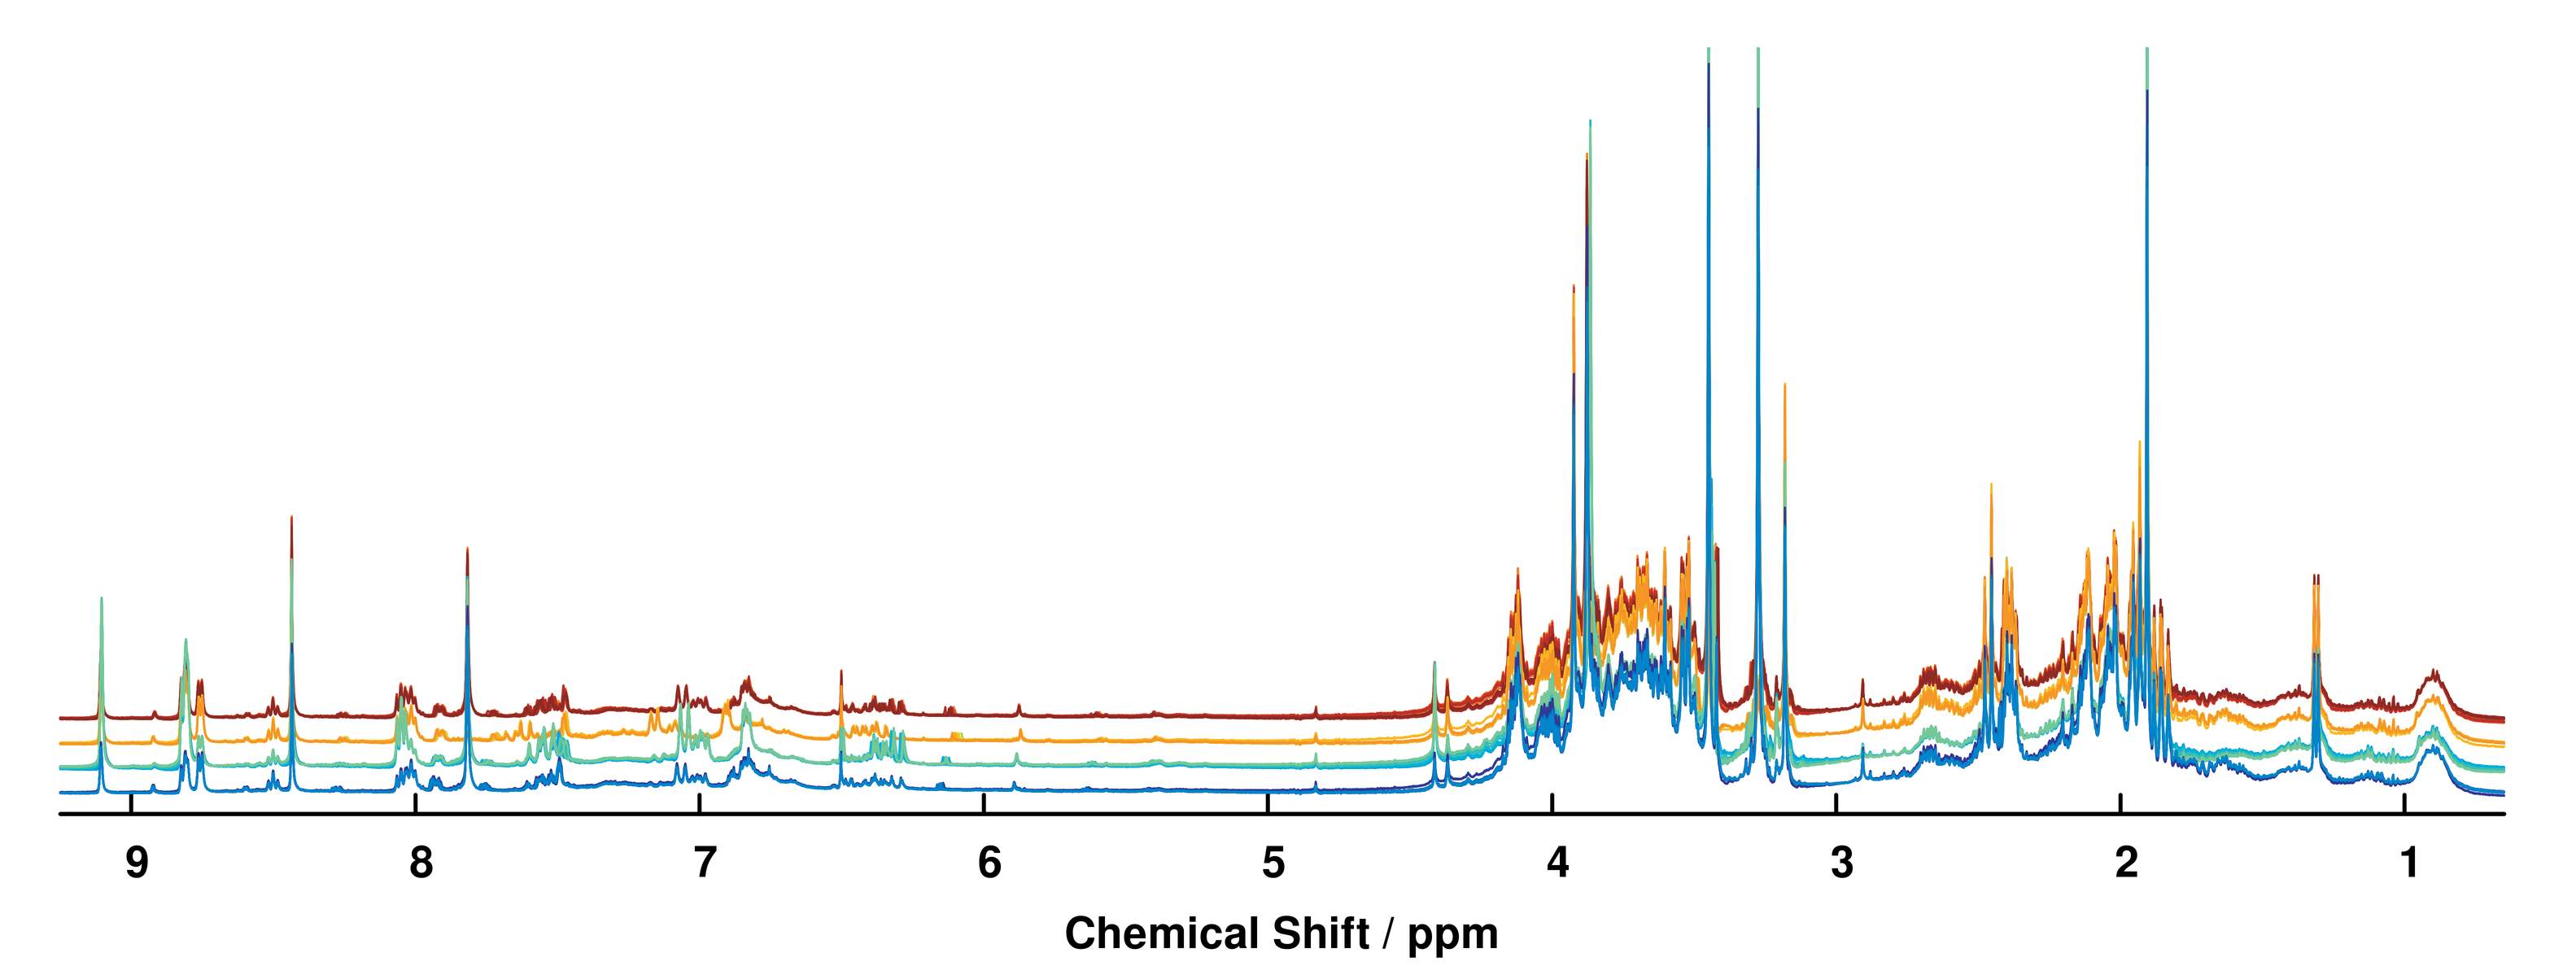
\includegraphics[width=6in]{figs/apps/02-spectra.png}
\caption
      [Processed \hnmr{} NMR Spectra of Coffee Roasts.]{
  {\bf Processed \hnmr{} NMR Spectra of Coffee Roasts.}
  \\
  Representative processed 1D \hnmr{} NMR spectra for all spectra of each
  coffee roast, acquired using the water-suppressed CPMG-$z$ pulse sequence
  and processed in MVAPACK. To reach this point, free induction decays were
  simply Fourier transformed and automatically phased. No manual phase
  corrections were applied after autophasing.
}
\label{figure.4.2}
\end{figure}

\begin{doublespace}
For principal component analysis (PCA), the dataset was normalized by the
method of probabilistic quotients (PQ, \cite{dieterle:anchem2006}) and
subjected to adaptive intelligent binning \cite{demeyer:anchem2008}.
Low-variation bins were automatically removed from the dataset
\cite{zhang:opin2008}, resulting in a final data matrix having 64 observations
and 284 variables. The data matrix was scaled to unit variance
\cite{vandenberg:bmcg2006} prior to NIPALS PCA modeling \cite{jolliffe2002},
which produced six significant components having cumulative \rsqx{} and
\qsq{} statistics of 0.9689 and $0.8965 \pm 0.0105$, respectively
\cite{eshghi:cils2014}.
\\\\
Linear discriminant analysis (LDA) was performed on the first three dimensions
of resulting PCA scores to yield a two-component model that best
captured the between-class variation present in the three orthonormal PCA
score vectors. LDA modeling yielded a model having a cumulative \rsqx{}
statistic of 0.9950 and cumulative \rsqy{} and \qsq{} statistics of 1.0.
Scores from the PCA model of the coffees \hnmr{} NMR spectral data, and
their corresponding LDA projection, are shown in \figref{4.3}{Figure 4.3}.
\end{doublespace}

\begin{figure}[ht!]
\includegraphics[width=6in]{figs/apps/03-pca-lda.png}
\caption
      [Principal Component Scores of the Coffees Spectra.]{
  {\bf Principal Component Scores of the Coffees Spectra.}
  \\
  PCA ({\bf A}) and LDA ({\bf B}) scores of the four coffee roasts. Red,
  green, blue and violet points represent dark, light, decaffeinated medium,
  and regular medium roasts, respectively. Ellipsoids and ellipses enclose
  the 95\% confidence intervals estimated by the sample means and covariances
  of scores from each class. Axis labels in panels ({\bf A}) and ({\bf B})
  indicate scores in PCA and LDA bases, respectively, and not the same set
  of scores.
}
\label{figure.4.3}
\end{figure}

\begin{doublespace}
For orthogonal projections to latent structures regression
(OPLS-R, \cite{trygg:jchemo2002}), the full-resolution dataset was aligned
using a per-class application of interval correlation-optimized shifting
(\emph{i}COshift, \cite{savorani:jmr2010}) and PQ normalization, resulting
in a final data matrix having 64 observations and 11,888 variables. The
Pareto-scaled data matrix was regressed by OPLS against a response vector
containing caffeine concentrations estimated by UV/Vis analysis of the four
coffee roasts, yielding a model with one predictive component and one
orthogonal component (\rsqxp{} = 0.5294, \rsqxo{} = 0.1288, \rsqy{} = 0.9822,
\qsq{} = $0.9502 \pm 0.0008$). CV-ANOVA significance testing returned a $p$
value equal to zero ($F$ = 2258.8) to within double-precision floating point
error, indicating a reliable model. The OPLS-R and LDA models were further
validated using response permutation tests having 1,000 iterations each. The
permutation tests of both models resulted in $p$ values less than 0.001 for
both \rsqy{} and \qsq{}, a further indication of high model reliability.
\end{doublespace}

\subsubsection{Validation against SIMCA-P+}

\begin{doublespace}
Correctness of the PCA and OPLS-R models generated by MVAPACK was verified by
exporting the final processed and treated data matrices from GNU Octave and
modeling them in SIMCA-P+ 13.0 (Umetrics AB, Umea, Sweden). The scores
extracted from SIMCA and MVAPACK were found to have coefficients of
determination (\rsq{}) of 0.999976 and 0.999989 for the PCA and OPLS models,
respectively. The ``imperfect'' non-unity values of \rsq{} reflect the fact
that SIMCA-P+ 13.0 only permits the export of scores with no more than four
decimal places.
\end{doublespace}

\begin{SCfigure}
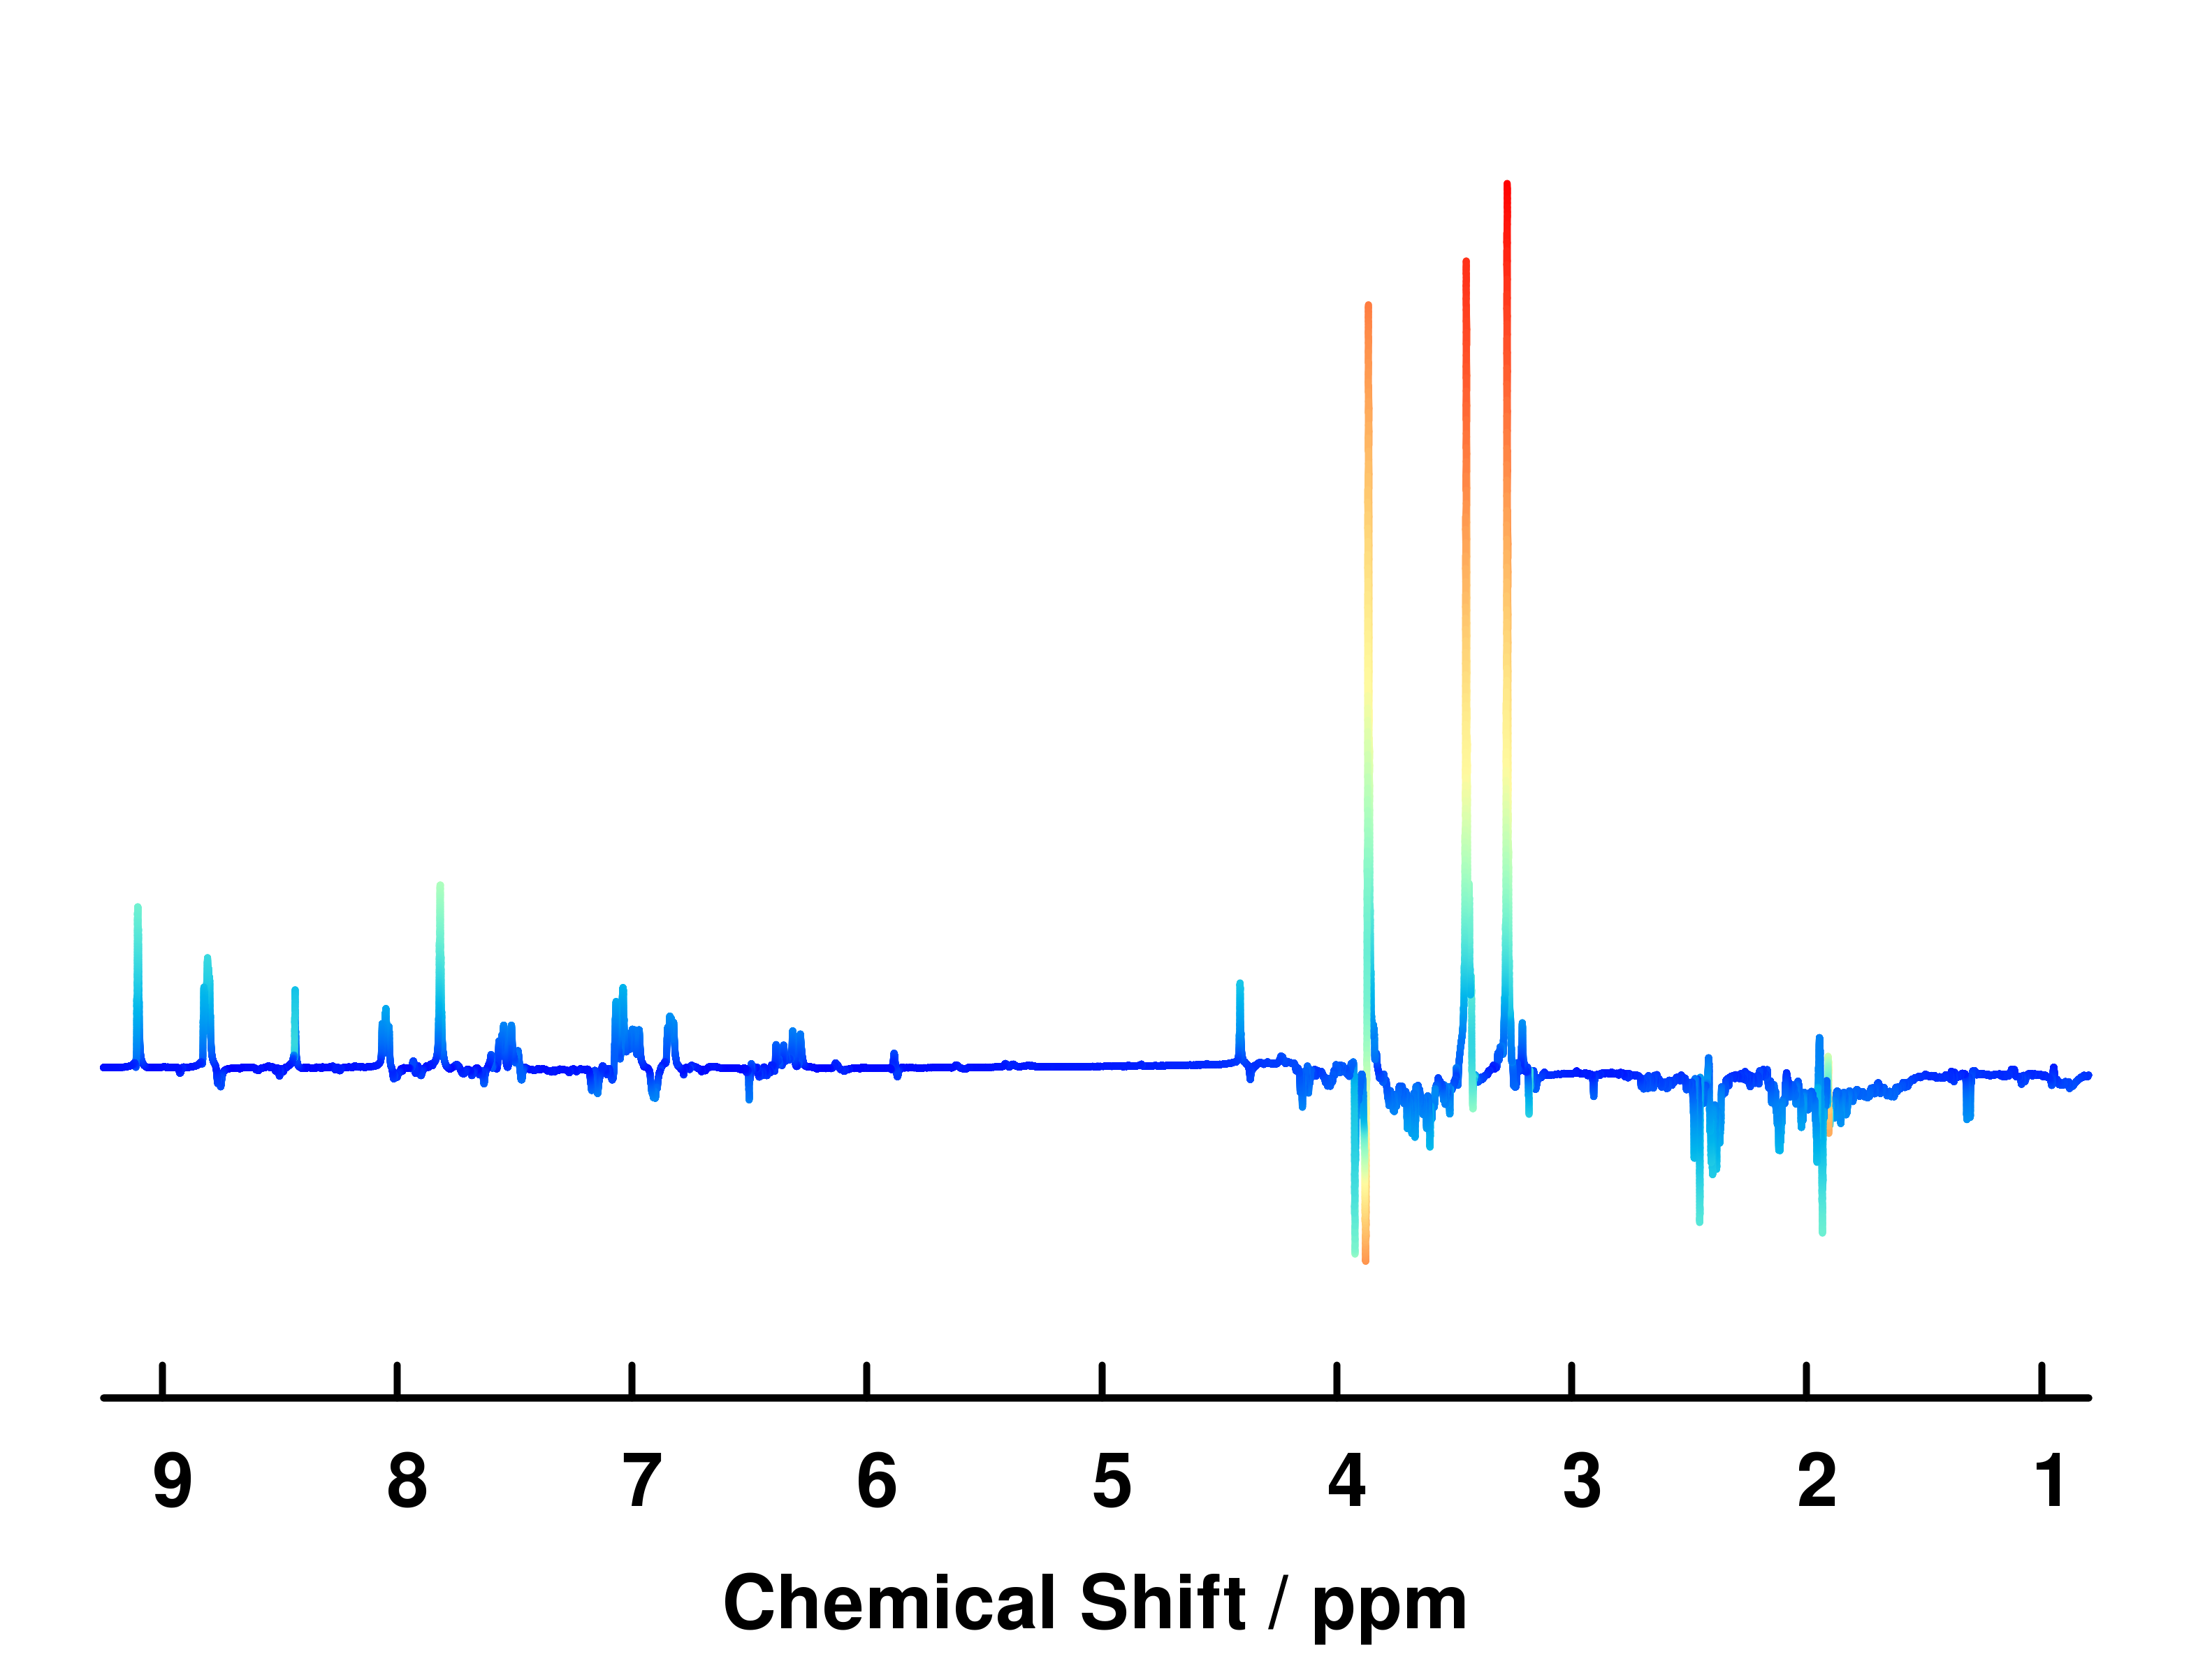
\includegraphics[width=3.25in]{figs/apps/04-oplsr-p.png}
\caption
      [Backscaled Coffees OPLS-R Model Loadings.]{
  {\bf Backscaled Coffees OPLS-R Model Loadings.}
  \\
  Backscaled OPLS-R predictive loadings of the four coffee roasts regressed
  according to estimated caffeine concentration. The pseudospectral nature of
  backscaled loadings facilitates analysis of model results by any
  spectroscopist. The four most intense positive positive peaks in the
  loadings pseudospectrum correspond directly to caffeine NMR resonances
  archived in the BMRB, indicating a fairly successful regression against
  caffeine concentration.
}
\label{figure.4.4}
\end{SCfigure}

\subsection{Results and Discussion}

\begin{doublespace}
Use of MVAPACK during analysis of the coffees dataset arguably facilitated
rapid identification of ideal processing, treatment and modeling parameters
during data handling. Use of automatic phase correction, adaptive intelligent
binning, and PQ normalization yielded a dataset in which three principal
components were sufficient to fully separate all classes in scores space,
and subsequent LDA modeling resulted in complete class separation in only
two components (\figref{4.3}{Figure 4.3}).
\\\\
As opposed to the PCA modeling procedure, which utilized binned spectra,
OPLS-R model training was performed using full-resolution 1D \hnmr{} NMR
spectra in order to reap the interpretive advantages of full-resolution
backscaled loadings (\figref{4.4}{Figure 4.4}). The availability of
\emph{i}COshift alignment \cite{savorani:jmr2010} in MVAPACK effectively
makes the modeling of full-resolution NMR spectral data possible by correcting
positional noise \cite{aberg:abc2009} in the spectra that corrupts the bilinear
nature of the data. By regressing the NMR data against estimates of caffeine
concentration obtained by UV/Vis spectroscopy (\figref{4.1}{Figure 4.1}),
a loading pseudo-spectrum of caffeine was obtained that matched almost
perfectly with spectral data deposited in the Biological Magnetic Resonance
Bank \cite{ulrich:nar2008}. It is conceivable that spectral features
co-extracted with caffeine in the loadings correspond to coffee bean
metabolites lost alongside caffeine during roasting or decaffeination.
\end{doublespace}

\begin{figure}[H]
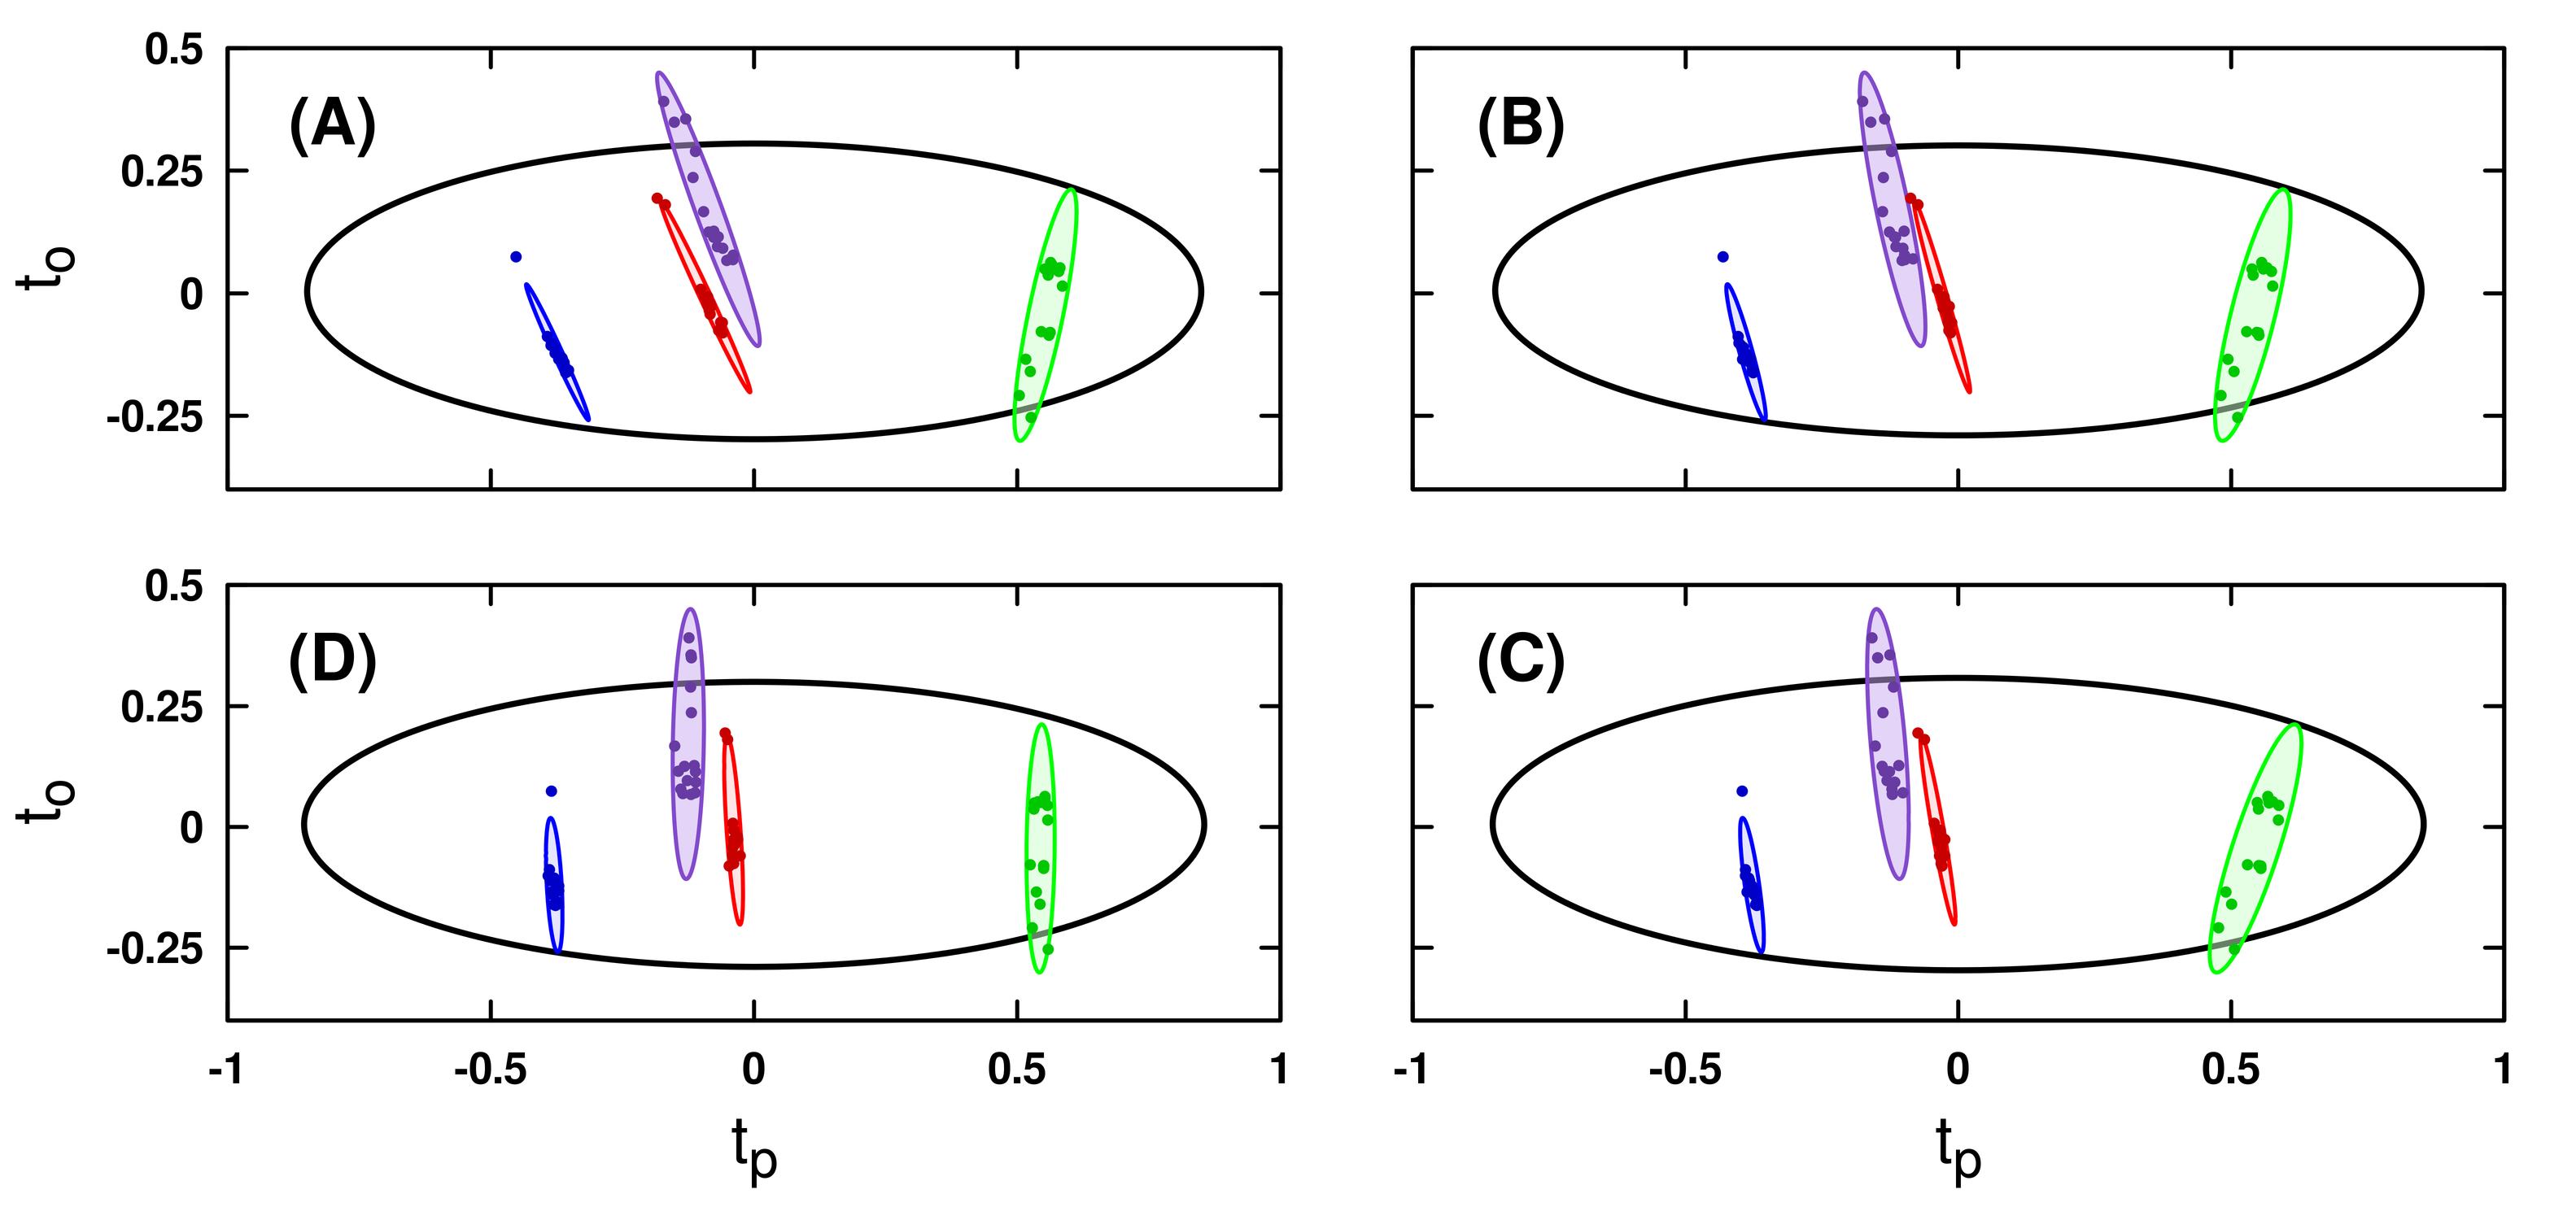
\includegraphics[width=6in]{figs/apps/05-oplsr-t.png}
\caption
      [Coffees OPLS-R Scores as Evidence of Overfit.]{
  {\bf Coffees OPLS-R Scores as Evidence of Overfit.}
  \\
  OPLS-R scores of the four coffee roasts, where each roast was regressed
  against its caffeine concentration estimated by UV/Vis absorbance
  spectroscopy. Scores in panels ({\bf A}) through ({\bf D}) were computed
  from models having 1 through 4 orthogonal components, respectively.
}
\label{figure.4.5}
\end{figure}

\begin{figure}[H]
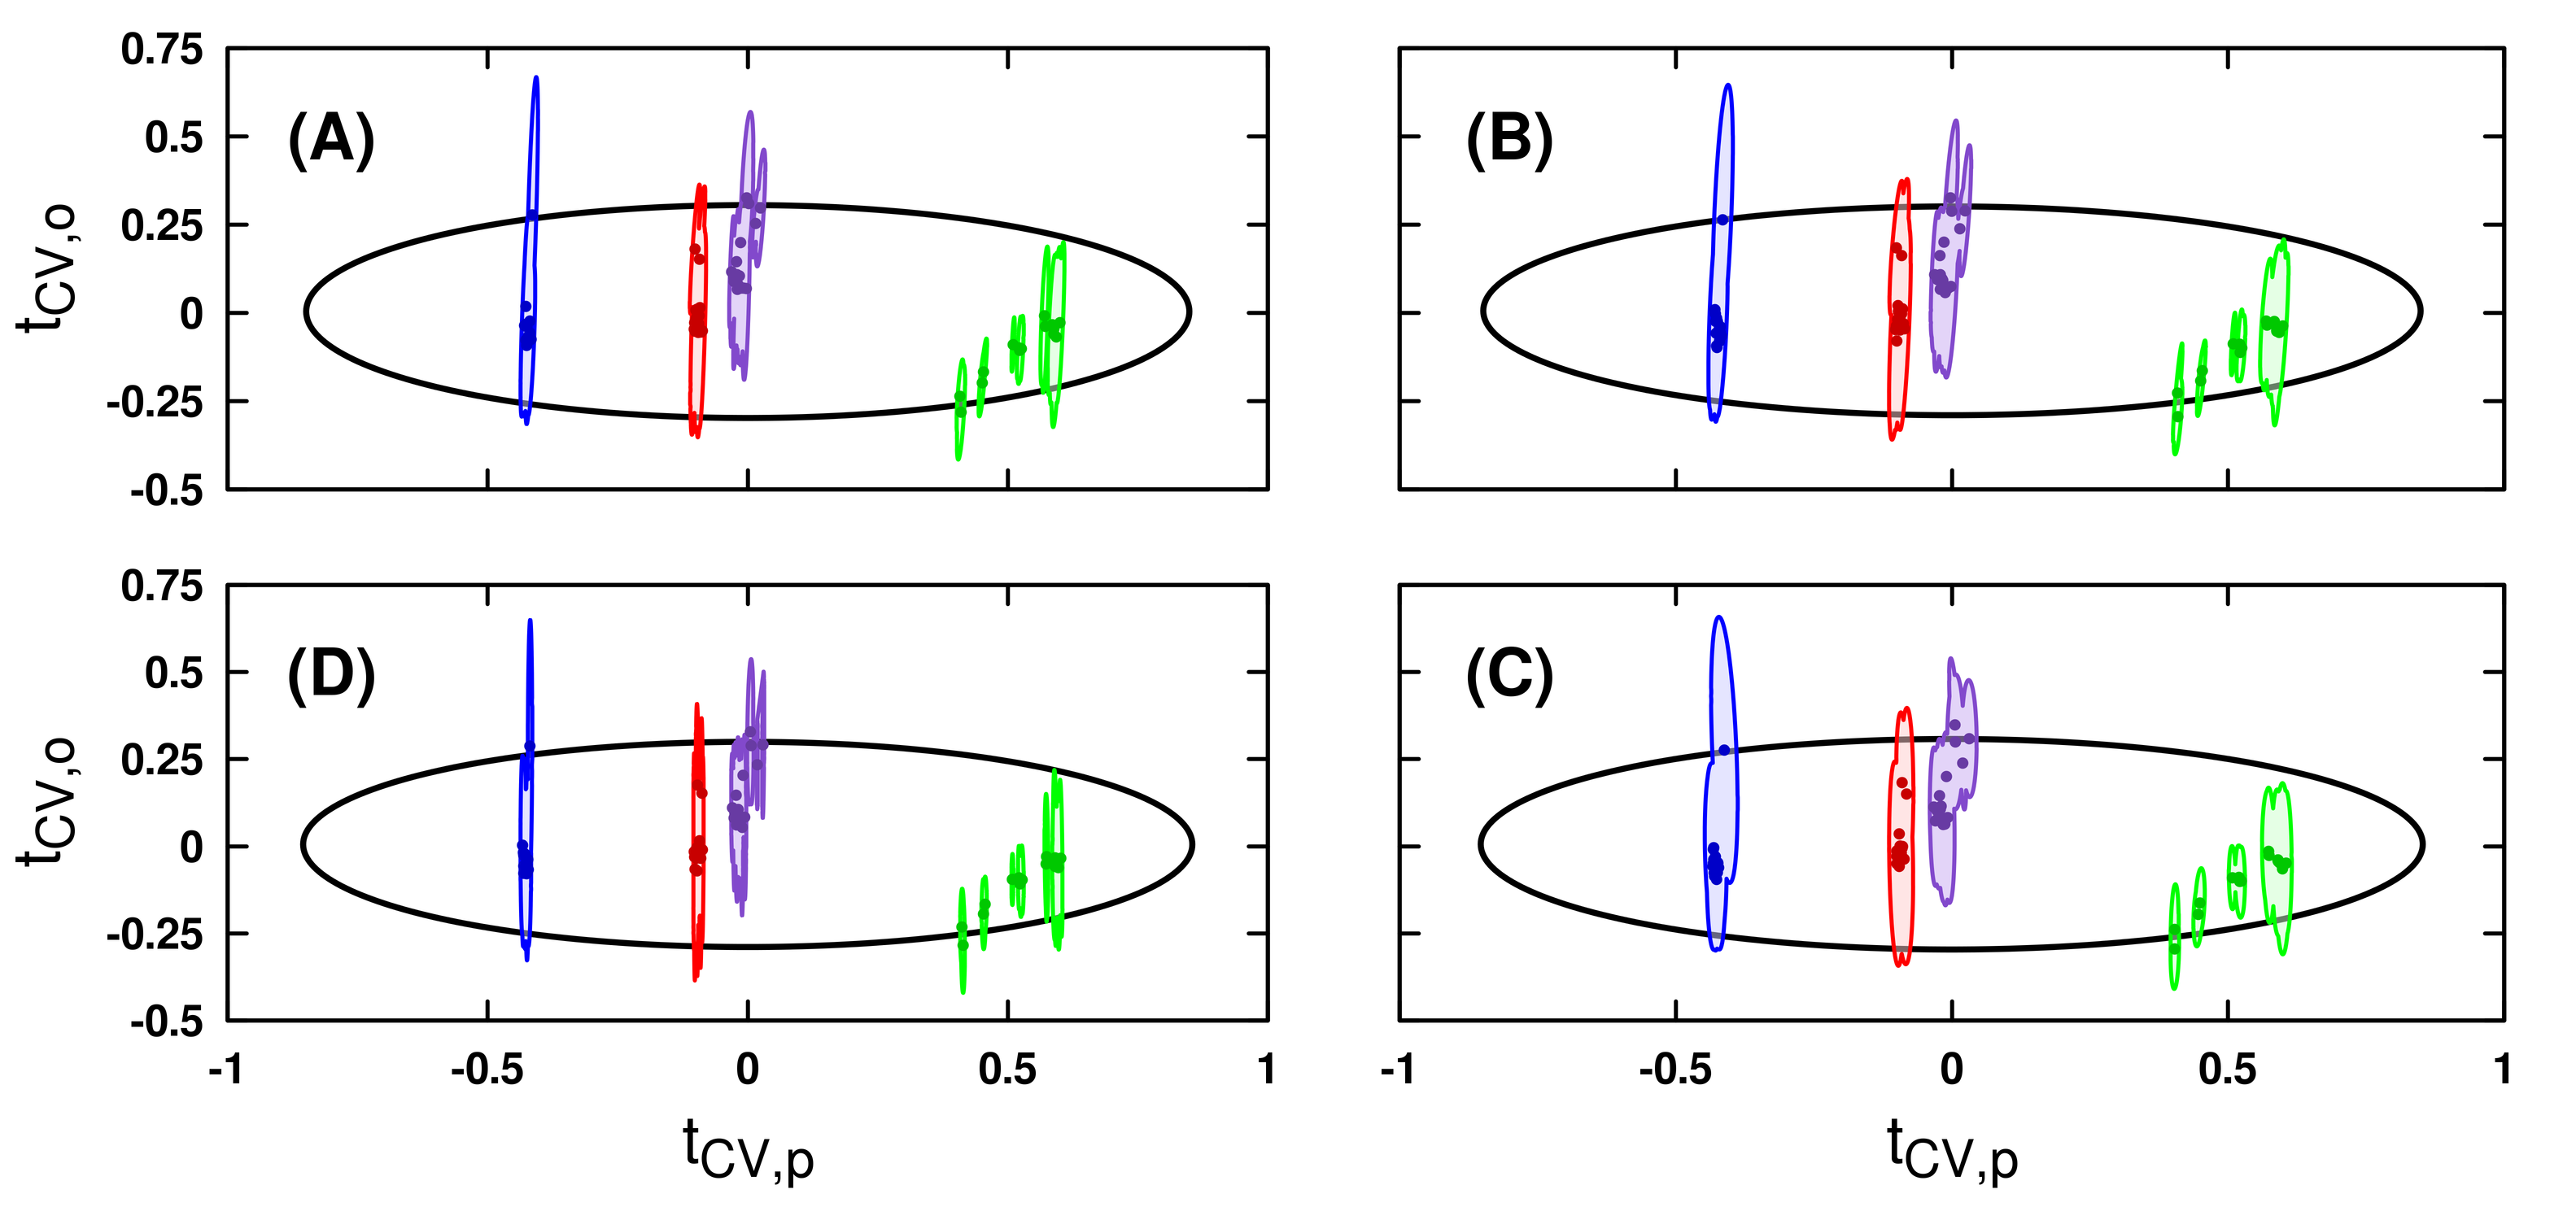
\includegraphics[width=6in]{figs/apps/06-oplsr-tcv.png}
\caption
      [Coffees OPLS-R Cross-validated Scores.]{
  {\bf Coffees OPLS-R Cross-validated Scores.}
  \\
  OPLS-R scores of the four coffee roasts, where each roast was regressed
  against its caffeine concentration, as in Figure 4.5. Mean score values
  and confidence ellipses for each observation were computed from 100
  iterations of seven-fold Monte Carlo internal cross-validation.
}
\label{figure.4.6}
\end{figure}

\begin{doublespace}
Notably, the UV/Vis-estimated caffeine concentration of the dark roast coffee
was slightly higher than that of the medium roast, which is contrary to
expectation given that the coffees were brewed using equal volumes of
grounds. However, OPLS-R of the NMR data using the estimated caffeine
concentrations correctly ranked the roasts according to expectation
(\figref{4.5}{Figure 4.5A}). When more orthogonal components were allowed
into the OPLS-R model, the dark roast again shifted to a higher caffeine
concentration, beautifully indicating the presence of overfitting
(\figref{4.5}{Figure 4.5B--D}). Monte Carlo cross-validated scores further
supported the fact that a $1+1$ OPLS model was the most appropriate
(\figref{4.6}{Figure 4.6}). Therefore, an OPLS-R model having only a single
orthogonal component was chosen, given the fact that it more faithfully
modeled the underlying NMR data at the expense of contradicting the more
uncertain UV/Vis measurements.
\\\\
Finally, no discernable difference was observed between the 1D \hnmr{} NMR
spectra acquired with and without $T_2$-filtering. Spectra collected on
in-house brewed coffee exhibited high levels of protein background signal,
which were readily suppressed using the CPMG-$z$ pulse sequence element. On
the other hand, the spectra of the four purchased roasts showed no such
background signal, possibly due to more correct brewing technique.
\end{doublespace}

\section{Fingerprinting of Joint \hnmr{} NMR and DI-ESI-MS Data}

\begin{doublespace}
Multiblock bilinear factorizations such as CPCA-W, MB-PLS and MB-OPLS provide
a powerful framework for analyzing a set of multivariate observations from
multiple analytical measurements containing potentially correlated variables
\cite{westerhuis:jchemo1997,westerhuis:jchemo1998,smilde:jchemo2003}. Such
algorithms provide analogous information to PCA, PLS and OPLS in situations
where extra knowledge is available to subdivide the measured variables into
multiple ``blocks''. As a result, the correlation structures of each block
\emph{and} the between-block correlations may be simultaneously utilized.
Due to the existence of common trends among all blocks, this use of
between-block correlations during modeling will ideally bring the model
loadings (latent variables) into better agreement with the true underlying
biochemistry (hidden variables). In short, multiblock algorithms provide an
ideal means of integrating 1D \hnmr{} NMR and direct injection electrospray
mass spectrometry (DI-ESI-MS) datasets for metabolic fingerprinting
\cite{xu:abc2013}.
\\\\
Consensus PCA (\hyperlink{subsection.3.5.4}{CPCA-W}),
Multiblock PLS (\hyperlink{subsection.3.5.5}{MB-PLS}), and
Multiblock OPLS (\hyperlink{subsection.3.5.6}{MB-OPLS}) were used to analyze
1D \hnmr{} NMR and DI-ESI-MS data collected on metabolite extracts from
human dopaminergic neuroblastoma cells (SK-N-SH) after different neurotoxin
treatments \cite{marshall:metab2015}. Each dataset was also individually
subjected to single-block modeling by PCA and PLS in order to highlight the
information gained by jointly modeling the data within multiblock frameworks.
\end{doublespace}

\subsection{Materials and Methods}

\subsubsection{NMR Acquisition and Processing}

\begin{doublespace}
NMR data were collected and processed according to previously described
procedures \cite{zhang:jiomic2013}. A Bruker Avance DRX 500 MHz spectrometer
equipped with a 5 mm inverse triple-resonance cryoprobe (\hnmr{}, \cnmr{},
\nnmr{}) with a $z$-axis gradient, a BACS-120 sample changer, and an automatic
tuning and matching accessory were utilized for automated NMR data collection.
Free induction decays were collected into 32,768 complex data points over a
spectral window of 2,342$\pm$2,741 ppm, using the SOGGY water suppression
pulse sequence (\emph{zgesgp}, \cite{hwang:jmr1995,nguyen:jmr2007}).
\\\\
Following acquisition, the 1D \hnmr{} NMR free induction decays were processed
in the MVAPACK toolbox \cite{worley:acscb2014}. A 1.0 Hz exponential
apodization fuction and a single round of zero-filling were applied prior to
Fourier transformation. Spectra were then automatically phased and normalized
using phase-scatter correction (PSC, \cite{worley:cils2014},
\hyperlink{chapter.6}{Chapter 6}). Finally, chemical shift regions
containing spectral baseline noise or solvent signals were manually removed.
Binning of the processed NMR spectra was performed using the Adaptive
Intelligent (AI) binning algorithm that avoids splitting signals into
multiple bins \cite{demeyer:anchem2008}.
\end{doublespace}

\subsubsection{MS Acquisition and Processing}

\begin{doublespace}
Mass spectra of the SK-N-SH metabolite extracts were acquired in positive ion
mode over a mass range of $m/z$ 50--1,200. Spectra were acquired for 30 s each
using the following source conditions: 2.5 kV electrospray capillary voltage,
60 V sampling cone voltage, 4.0 V extraction voltage, $80^\circ$C source
temperature, $250^\circ$C desolvation temperature, 500 L/h desolvation gas
flow rate, and 15 $\mu$L/min injection flow rate.
\\\\
The initial stages of mass spectral data processing were performed using
MassLynx V4.1 (Waters Corp., Milford, MA). A background subtraction was
performed on all spectra: reference spectra of either paraquat,
1-methyl-4-phenylpyridinium (MPP$^+$), rotenone, or 6-hydroxydopamine (6-OHDA)
in H$_2$O/CH$_3$OH/HCO$_2$H (49.75:49.75:0.5) at 10 ppm were used as
backgrounds. Background subtraction of each spectrum was performed in a
class-dependent manner (e.g. the MPP$^+$ reference mass spectrum was used as
background for MPP$^+$-treated cell samples). As a result, mass spectral
signals from the drugs themselves were guaranteed to not influence subsequent
analyses. The background-subtracted mass spectra were then loaded into MVAPACK
for binning and normalization. All mass spectra were linearly re-interpolated
onto a common axis that spanned from $m/z$ 50--1,200 in 0.003 $m/z$ steps,
resulting in 383,334 variables prior to processing. Based on the low
probability of observing a metabolite in the mass range $m/z$ 1,100--1,200,
the region was removed prior to binning. Mass spectra were uniformly binned
using a bin width of 0.5 $m/z$, resulting in a data matrix of 2,095 variables.
Finally, the MS data matrix observations were normalized using probabilistic
quotient (PQ) normalization \cite{dieterle:anchem2006}.
\end{doublespace}

\subsubsection{Multivariate Statistical Analysis}

\begin{doublespace}
Using functions available in the latest version of MVAPACK, the NMR and MS
data were joined into a single multiblock data structure and modeled using
CPCA-W, MB-PLS and MB-OPLS. Both blocks were scaled to unit variance prior
to modeling, and equal contribution of each block to the models (fairness)
was ensured by further scaling each block by the square root of its variable
count \cite{smilde:jchemo2003}. For the purposes of comparison, PCA and PLS
models of the independent NMR and MS data matrices were also constructed.
All PLS models were trained on a binary discriminant response matrix
(i.e. PLS-DA), in which untreated cells were assigned to one class,
and all neurotoxin-treated cells were assigned to a second class.
\end{doublespace}

\subsubsection{Cross-validation of Multivariate Models}

\begin{doublespace}
Initially, all PCA and CPCA-W models were internally cross-validated using a
leave-one-out (LOOCV) procedure in MVAPACK during model training
\cite{eshghi:cils2014}. A subsequent set of PCA models was trained and
cross-validated using a Monte Carlo seven-fold (MCCV) procedure that
produced less optimistic \qsq{} statistics. All PLS-DA, MB-PLS-DA and
MB-OPLS-DA models were internally cross-validated using a Monte Carlo
seven-fold procedure \cite{wold:cils2001}. All MCCV rounds involved 50
iterations per tested model component. The results of cross-validation
were summarized by per-component \qsq{} statistics, and the number of model
components was chosen such that the cumulative \qsq{} was a strictly increasing
function of component count. Response permutation tests of all supervised
models were performed with 1,000 permutations each to assess the statistical
significance of \rsqy{} and \qsq{} values \cite{westerhuis:metab2008a}.
CV-ANOVA significance tests \cite{eriksson:jchemo2008} were also performed
to supplement the results of the permutation tests.
\end{doublespace}

\begin{SCfigure}
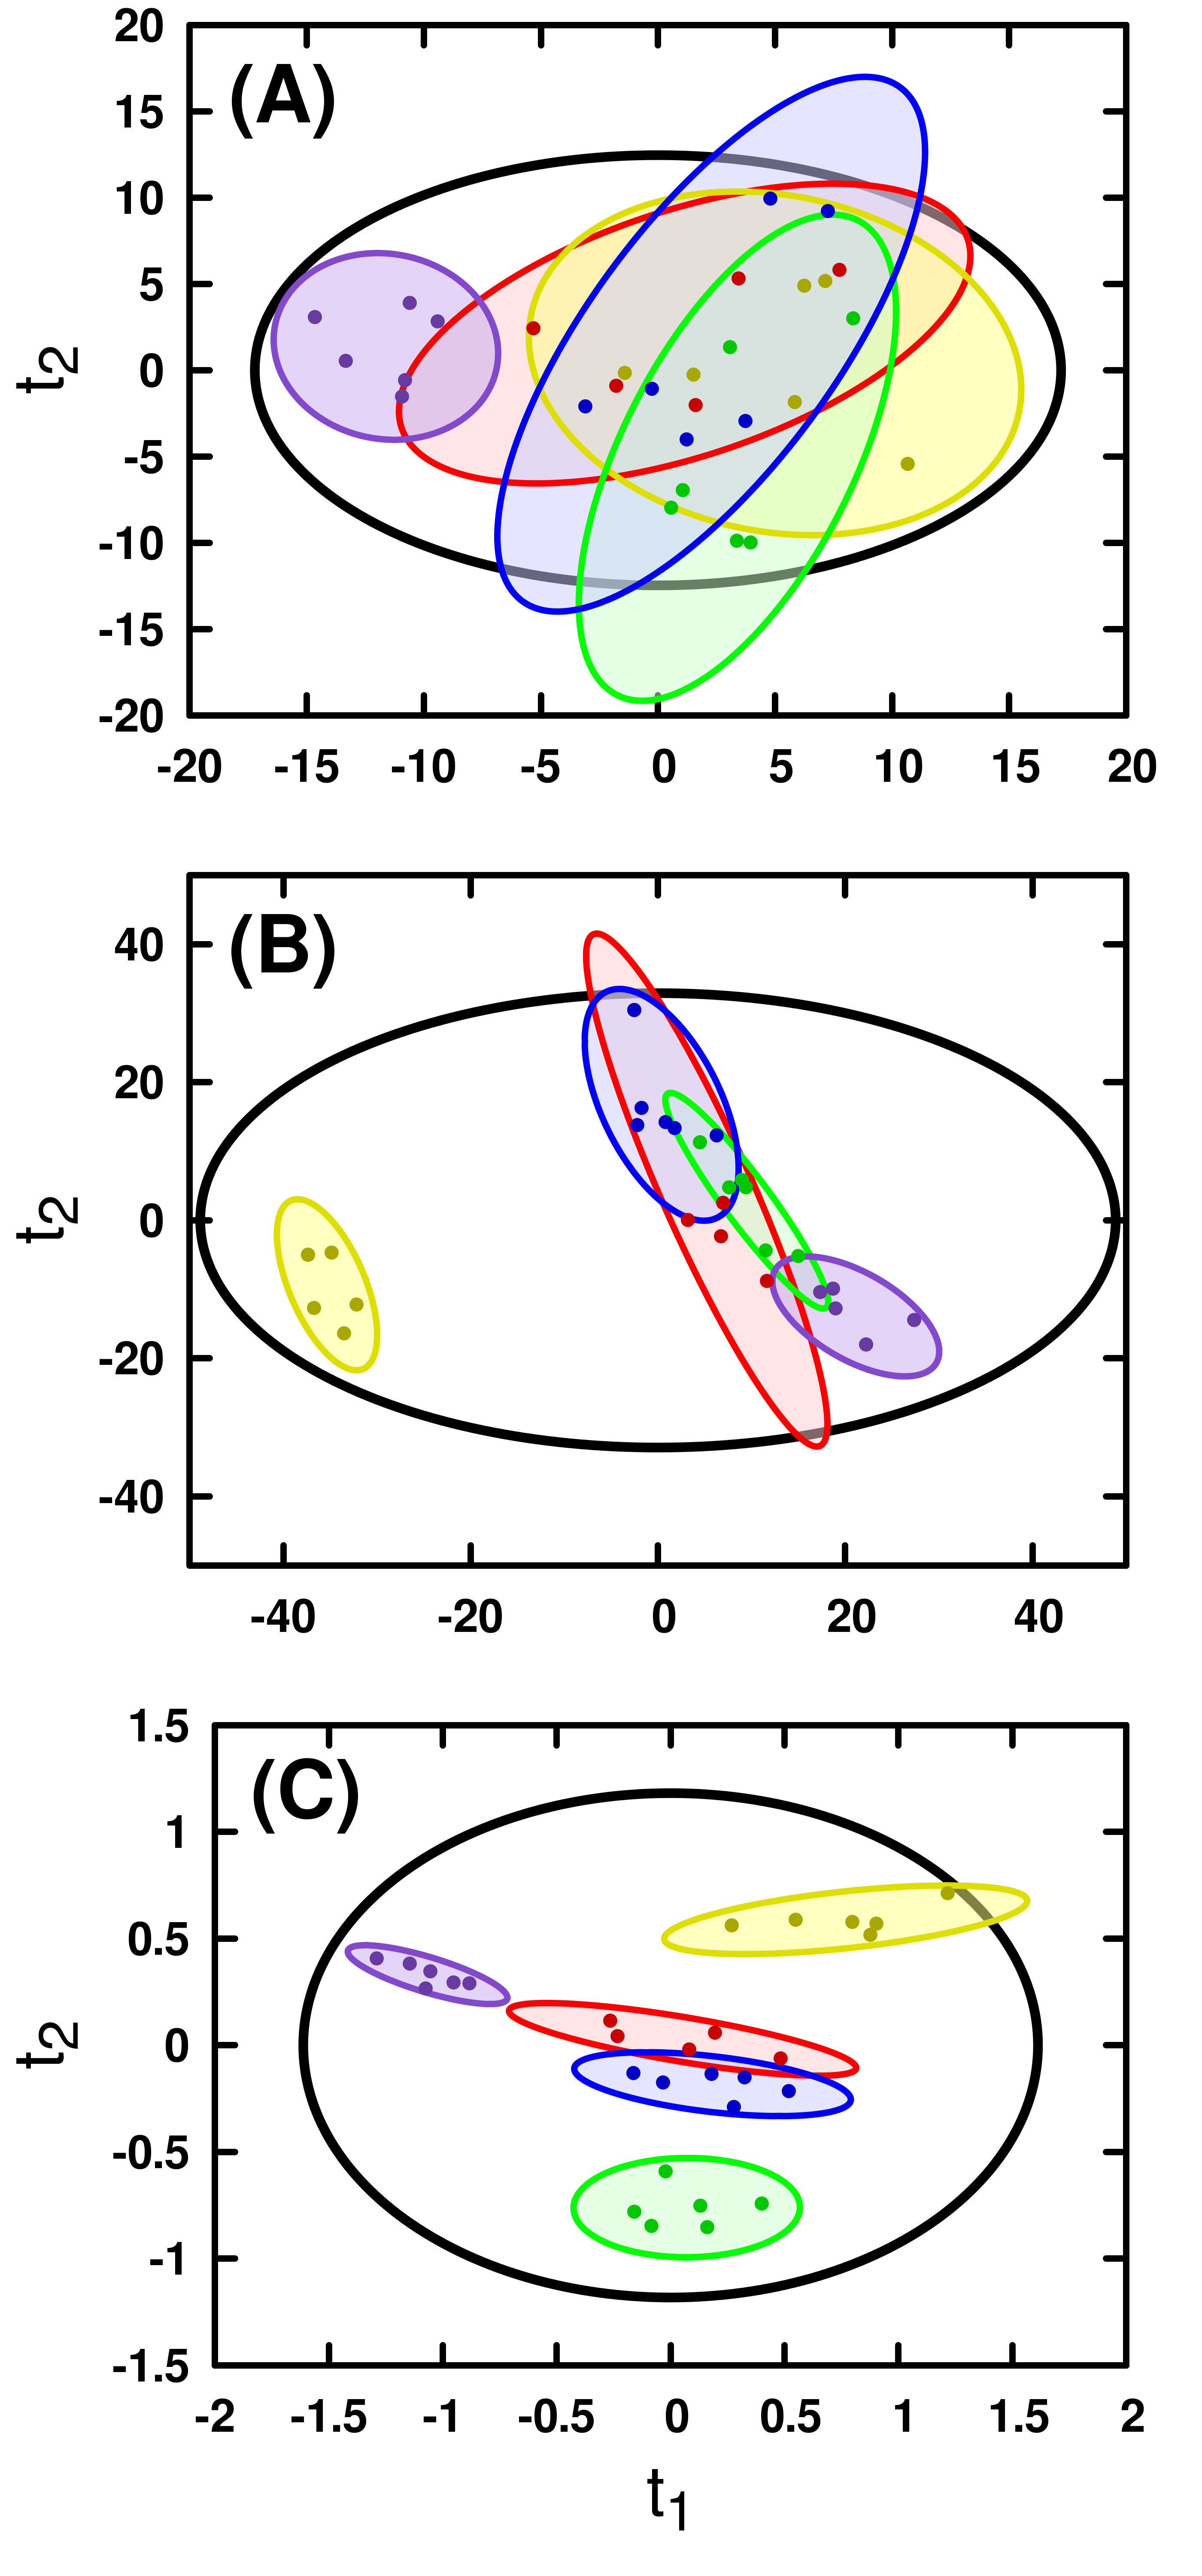
\includegraphics[width=3.25in]{figs/apps/07-mbpca-t.png}
\caption
      [Comparison of PCA and MB-PCA Scores.]{
  {\bf Comparison of PCA and MB-PCA Scores.}
  \\
  Scores generated from ({\bf A}) PCA of \hnmr{} NMR in vacuo, ({\bf B}) PCA
  of DI-ESI-MS in vacuo, and ({\bf C}) MB-PCA of \hnmr{} NMR and DI-ESI-MS.
  Separations between classes are increased upon combination of the two
  data matrices via MB-PCA. Yellow, red, green, violet and blue scores
  correspond to the control, 6-OHDA, MPP$^+$, paraquat and rotenone classes,
  respectively.
}
\label{figure.4.7}
\end{SCfigure}

\begin{SCfigure}
\includegraphics[width=2.2in]{figs/apps/08-mbpca-d.png}
\caption
      [Dendrograms of PCA and MB-PCA Scores.]{
  {\bf Dendrograms of PCA and MB-PCA Scores.}
  \\
  Dendrograms computed from scores-space class separations
  \cite{worley:abio2013} in the in vacuo PCA and MB-PCA models. Panels
  ({\bf A--C}) correspond to scores in panels ({\bf A--C}) in Figure 4.7,
  above.
}
\label{figure.4.8}
\end{SCfigure}

\subsection{Results and Discussion}

\subsubsection{Classical Modeling}

\begin{doublespace}
PCA of the binned NMR data matrix ($N$ = 29, $K$ = 159) resulted in 10
principal components having cumulative \rsqx{} and \qsq{} statistics of
0.9485 and 0.4591, respectively, based on LOOCV. Overall, no patterns were
readily discernable in the NMR PCA scores (\figref{4.7}{Figure 4.7A}) due to
high within-class variation in the data. However, scores for paraquat treatment
were found to significantly separate from all other classes ($p < 0.002$)
along the first principal component. Scores from PCA of the binned MS data
matrix ($N$ = 29, $K$ = 2,095) were found to exhibit markedly less within-class
variation compared to the NMR data (\figref{4.7}{Figure 4.7B}). Using LOOCV,
three significant components were identified from the binned MS data, yielding
fairly low cumulative \rsqx{} and \qsq{} statistics of 0.3397 and 0.1590.
While paraquat treatment still separated from other drug treatments in MS
PCA scores space, the greatest separations were observed between treated
and untreated (control) cells ($p < \times 10^{-9}$). These differing
patterns of separation in NMR and MS PCA scores suggested that multiblock
analyses could provide further information, ideally separating both control
and paraquat scores from all other classes. \figref{4.8}{Figure 4.8} contains
dendrograms of scores-space class separation for each scores plot in
\figref{4.7}{Figure 4.7}.
\\\\
Per-component \qsq{} statistics computed from LOOCV of the NMR and MS PCA
models suggested fairly marginal model reliability at component counts greater
than one, so follow-up analyses were performed using MCCV on the same data
matrices to obtain less optimistic estimates of reliability. In both cases,
MCCV produced single-component PCA models, indicating that the LOOCV had
substantially over-estimated the number of principal components in each
matrix. A comparison of the resulting \qsq{} statistics from LOOCV and MCCV
is shown in \figref{4.9}{Figure 4.9}.
\\\\
PLS-DA of the full-resolution NMR ($N$ = 29, $K$ = 16,138) and
MS ($N$ = 29, $K$ = 2,095) data matrices both resulted in two-component models.
With the exception of the algorithmically forced separation between control
and treatment classes, similar clustering patterns were observed when compared
to the PCA scores (\figref{4.10}{Figure 4.10A--B}). MCCV results from the
NMR ($R^2_Y = 0.9519, Q^2 = 0.7303 \pm 0.0517$) and
MS ($R^2_Y = 0.9951, Q^2 = 0.9440 \pm 0.01142$) PLS-DA models indicated
reasonable levels of response fit and predictive ability. Further validation
by CV-ANOVA \cite{eriksson:jchemo2008} indicated reliable models with $p$
values of 0.002 and $9.8 \times 10^{-6}$ for NMR and MS data, respectively.
Response permutation tests for both PLS-DA models returned $p < 0.001$,
supporting the CV-ANOVA test results.
\end{doublespace}

\begin{SCfigure}
\includegraphics[width=3.25in]{figs/apps/09-rqpca.png}
\caption
      [Comparison of LOOCV and MCCV \qsq{} Statistics for PCA.]{
  {\bf Comparison of LOOCV and MCCV \qsq{} Statistics for PCA.}
  \\
  \rsq{} (red), $Q^2_{\mathrm{LOOCV}}$ (green) and $Q^2_{\mathrm{MCCV}}$ (blue)
  statistics from ({\bf A}) PCA of \hnmr{} NMR in vacuo, ({\bf B}) PCA of
  DI-ESI-MS in vacuo, and ({\bf C}) MB-PCA of \hnmr{} NMR and DI-ESI-MS.
  In all cases, MCCV indicates that both datasets contain a single significant
  principal component, while LOOCV over-estimates the number of significant
  components.
}
\label{figure.4.9}
\end{SCfigure}

\begin{SCfigure}
\includegraphics[width=3.25in]{figs/apps/10-mbpls-t.png}
\caption
      [Comparison of PLS-DA and MB-PLS-DA Scores.]{
  {\bf Comparison of PLS-DA and MB-PLS-DA Scores.}
  \\
  Cross-validated scores generated from ({\bf A}) PLS-DA of \hnmr{} NMR in
  vacuo, ({\bf B}) PLS-DA of DI-ESI-MS in vacuo, and ({\bf C}) MB-PLS-DA of
  \hnmr{} NMR and DI-ESI-MS. Consensus directions in MB-PLS-DA scores space
  show decreased rotation during cross-validation when compared to PLS-DA
  scores of the in vacuo PCA model. Yellow, red, green, violet and blue scores
  correspond to the control, 6-OHDA, MPP$^+$, paraquat and rotenone classes,
  respectively.
}
\label{figure.4.10}
\end{SCfigure}

\subsubsection{Multiblock Modeling}

\begin{doublespace}
Identification of consensus directions in the NMR and MS data matrices that
maximally captured overall variation (MB-PCA) or response correlations (MB-PLS)
resulted in more informative models than those calculated against either NMR
or MS in vacuo. Using MB-PCA with LOOCV, five significant components were
identified ($Q^2 = 0.2322$) that cumulatively explained comparable amounts
of variation in the NMR ($R^2_X = 0.8528$) and MS ($R^2_X = 0.5015$) blocks
relative to the individual PCA models. As expected, MB-PCA combined the
information from both blocks to dramatically increase class separations in
super-scores space (\figref{4.7}{Figure 4.7C}). More specifically, both
control and paraquat classes were separated from other neurotoxin treatments,
predominantly along the first principal component. Furthermore, MPP$^+$
treatment exhibited significant separation from 6-OHDA and rotenone
treatments, which was not expected from examination of the individual
NMR or MS PCA scores.
\end{doublespace}

\begin{figure}[ht!]
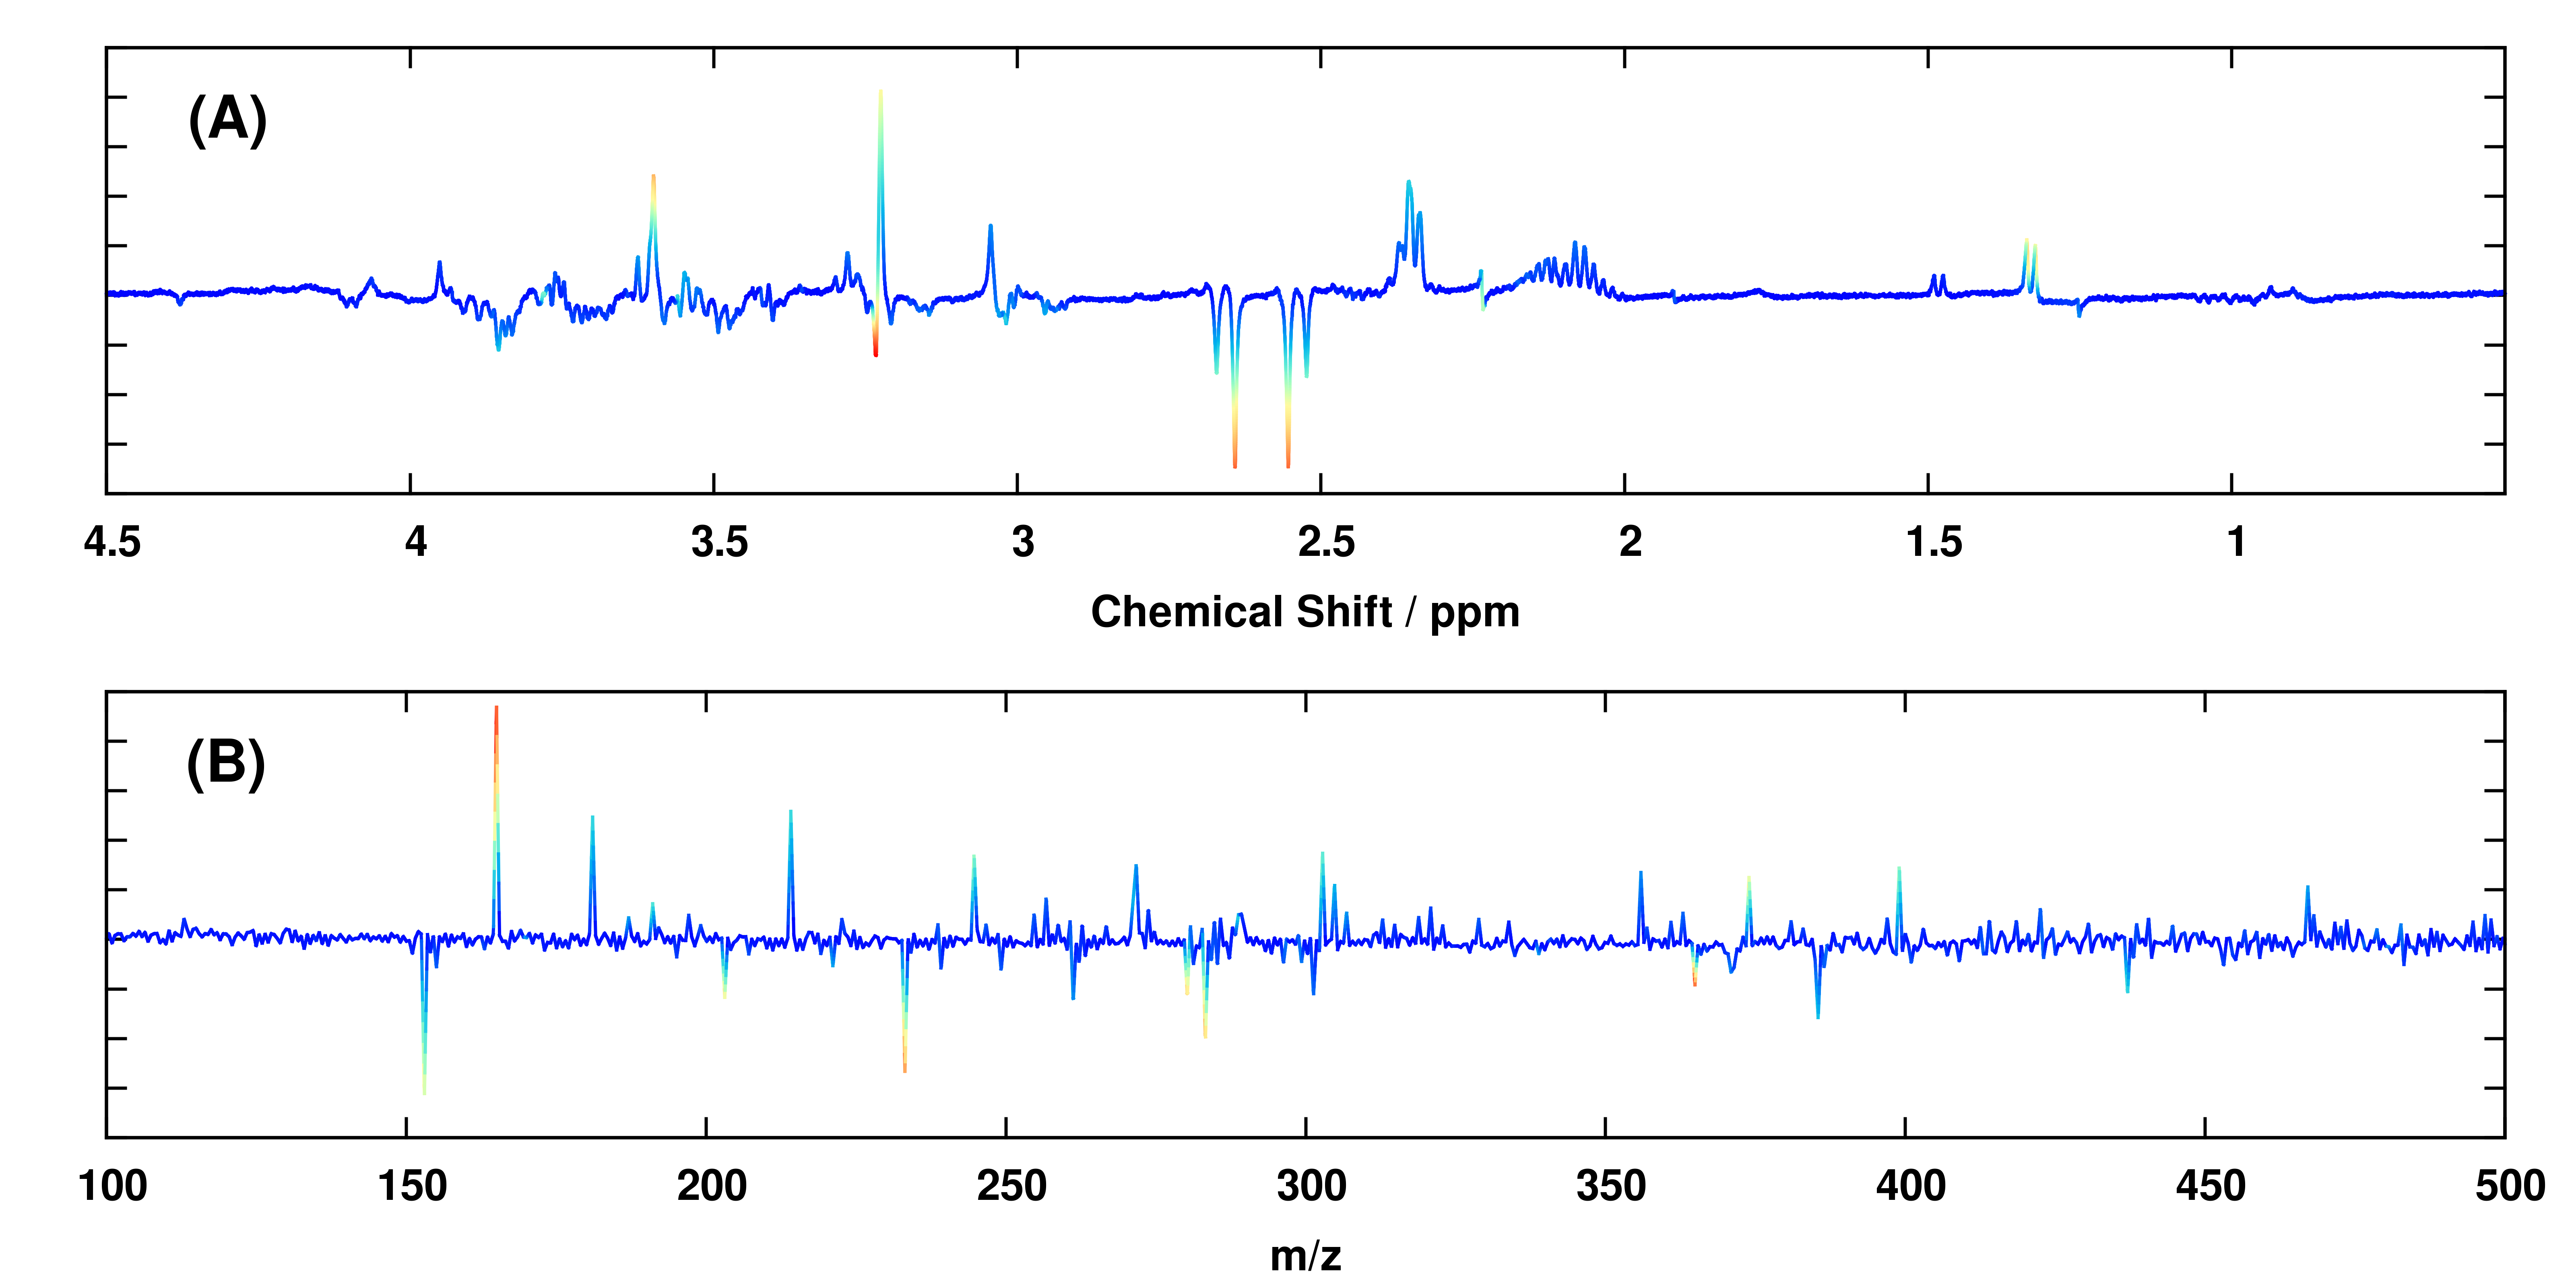
\includegraphics[width=6in]{figs/apps/11-mbpls-p.png}
\caption
      [Backscaled NMR and MS Block Loadings.]{
  {\bf Backscaled NMR and MS Block Loadings.}
  \\
  Backscaled ({\bf A}) \hnmr{} NMR block and ({\bf B}) DI-ESI-MS block loadings
  from MB-PLS-DA. Comparison of the above panels to those from MB-OPLS-DA
  (Figures 4.12, 4.13) reveals the mixed predictive and orthogonal variation
  present in MB-PLS loadings. It is also important to note that a second
  PLS component exists, and thus complete interpretation of the joint NMR
  and MS data requires simultaneous examination of \emph{two} sets of
  block loadings.
}
\label{figure.4.11}
\end{figure}

\begin{doublespace}
Subsequent re-evaluation of the MB-PCA model's reliability using MCCV reduced
the number of expected significant components to two
(\figref{4.9}{Figure 4.9C}). However, secondary and higher
components' \qsq{} statistics were still found to be
statistically indistinguishable from zero, which further suggests that only
one principal direction exists in the binned NMR and MS data matrices that
captures any substantial variation.
\end{doublespace}

\begin{figure}[ht!]
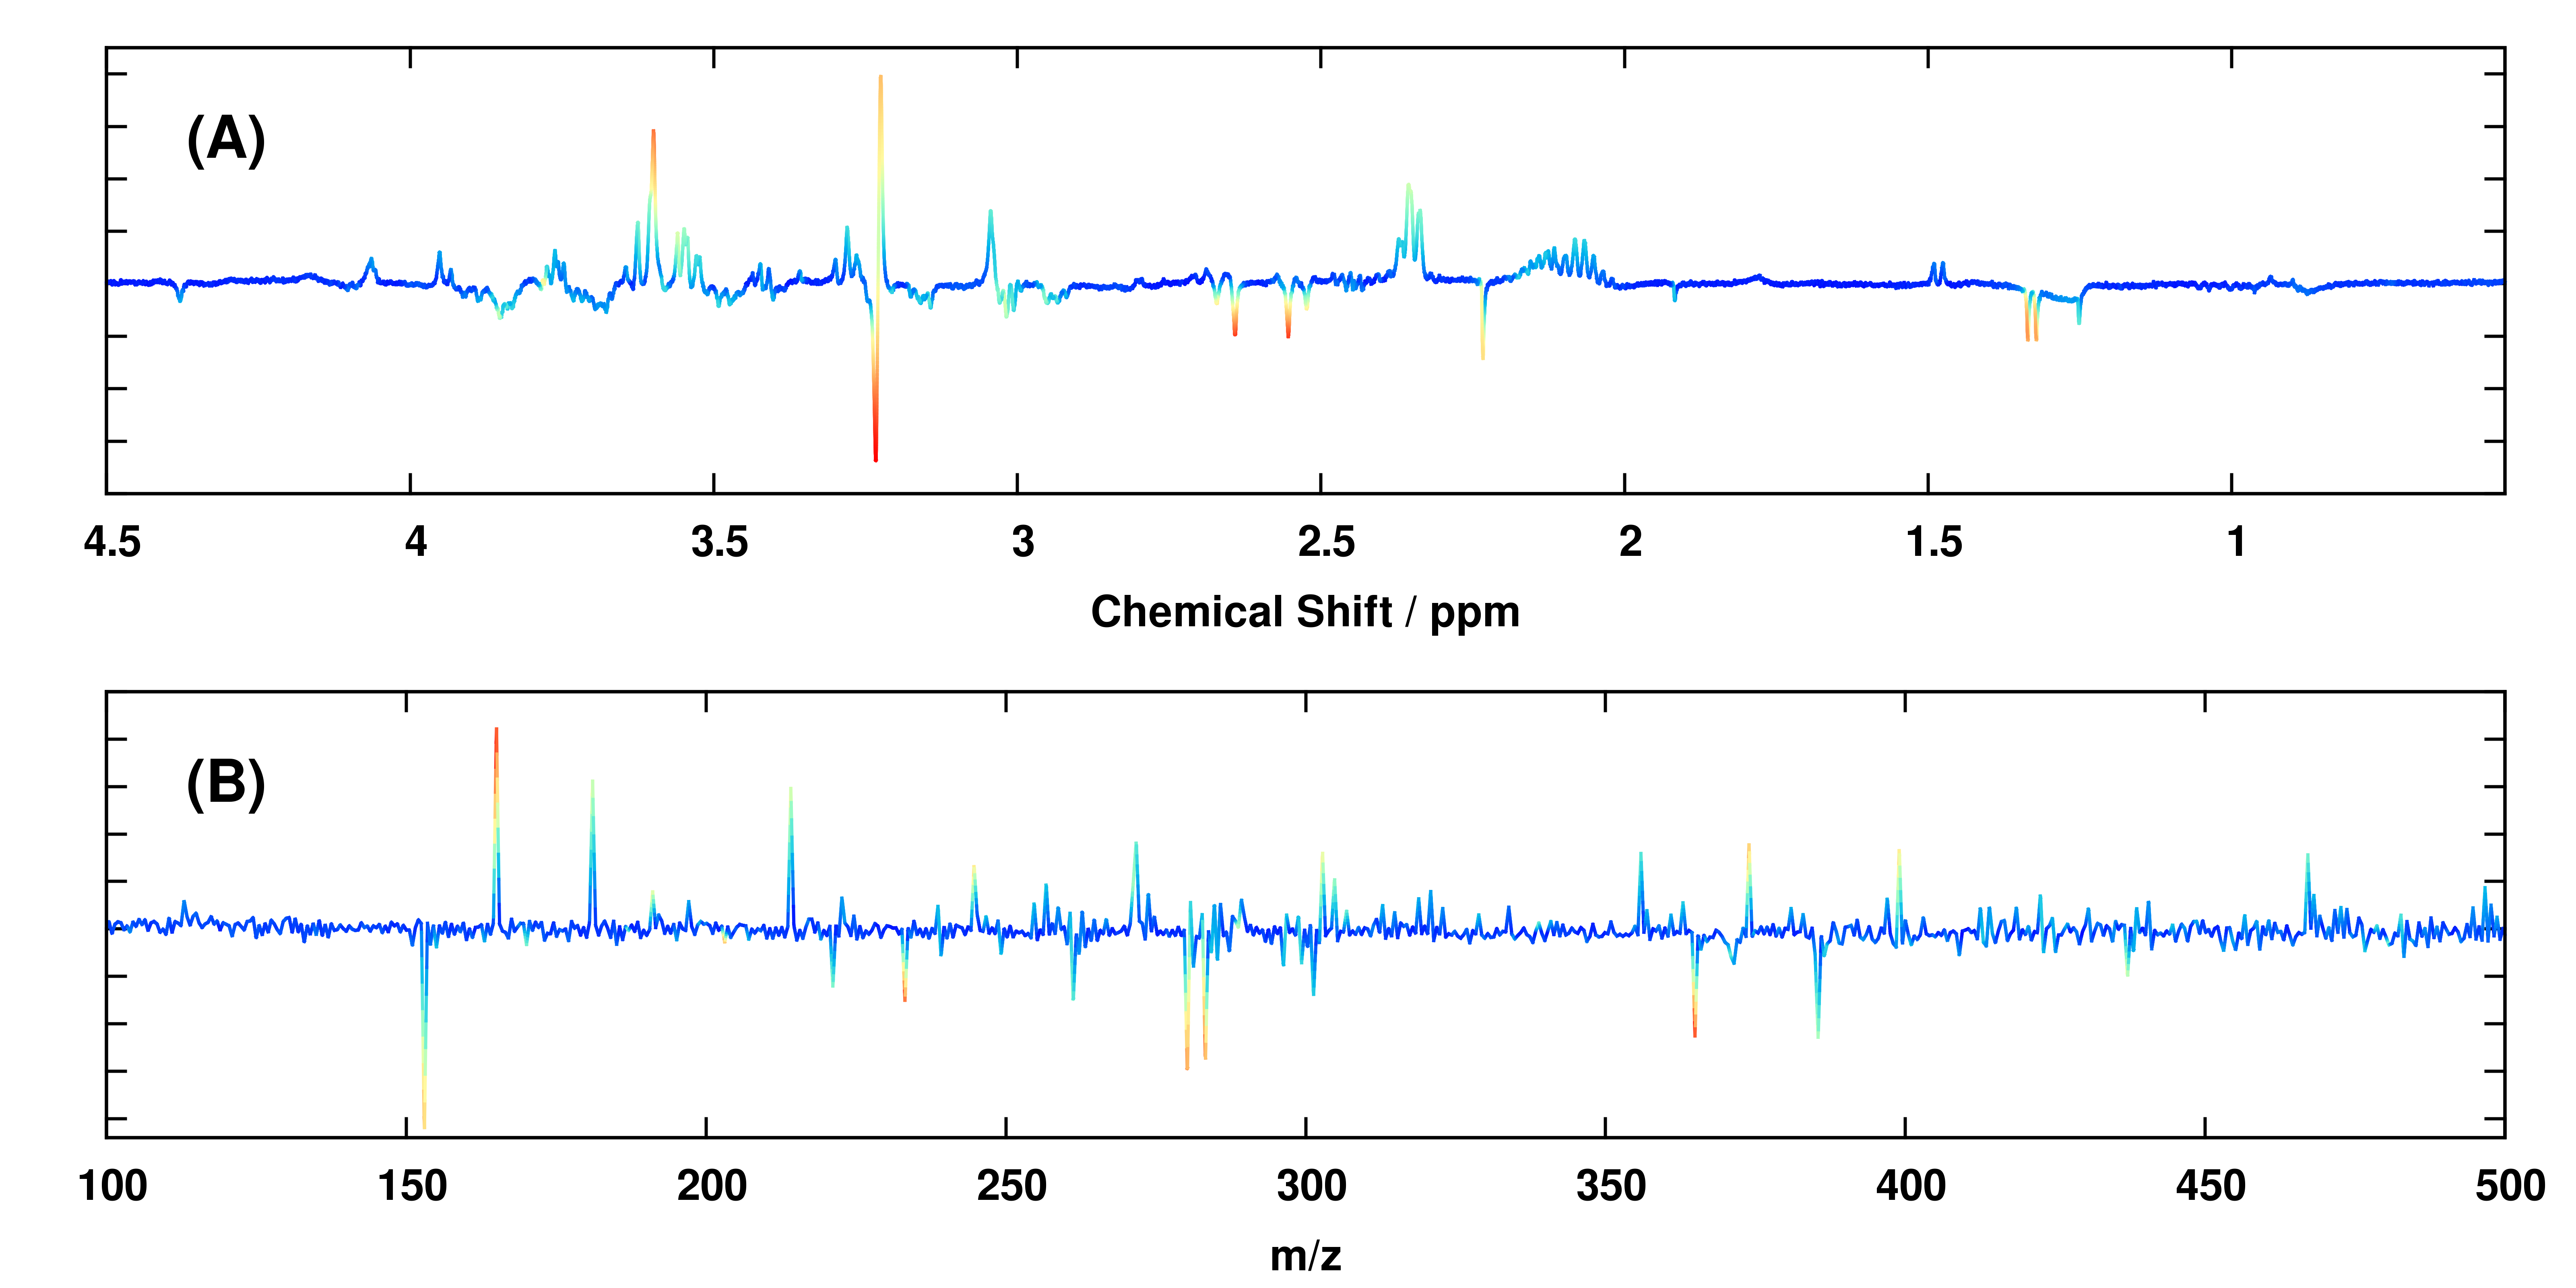
\includegraphics[width=6in]{figs/apps/12-mbopls-p.png}
\caption
      [Backscaled NMR and MS Predictive Block Loadings.]{
  {\bf Backscaled NMR and MS Predictive Block Loadings.}
  \\
  Backscaled predictive ({\bf A}) \hnmr{} NMR block and ({\bf B}) DI-ESI-MS
  block loadings from MB-OPLS-DA.
}
\label{figure.4.12}
\end{figure}

\begin{figure}[ht!]
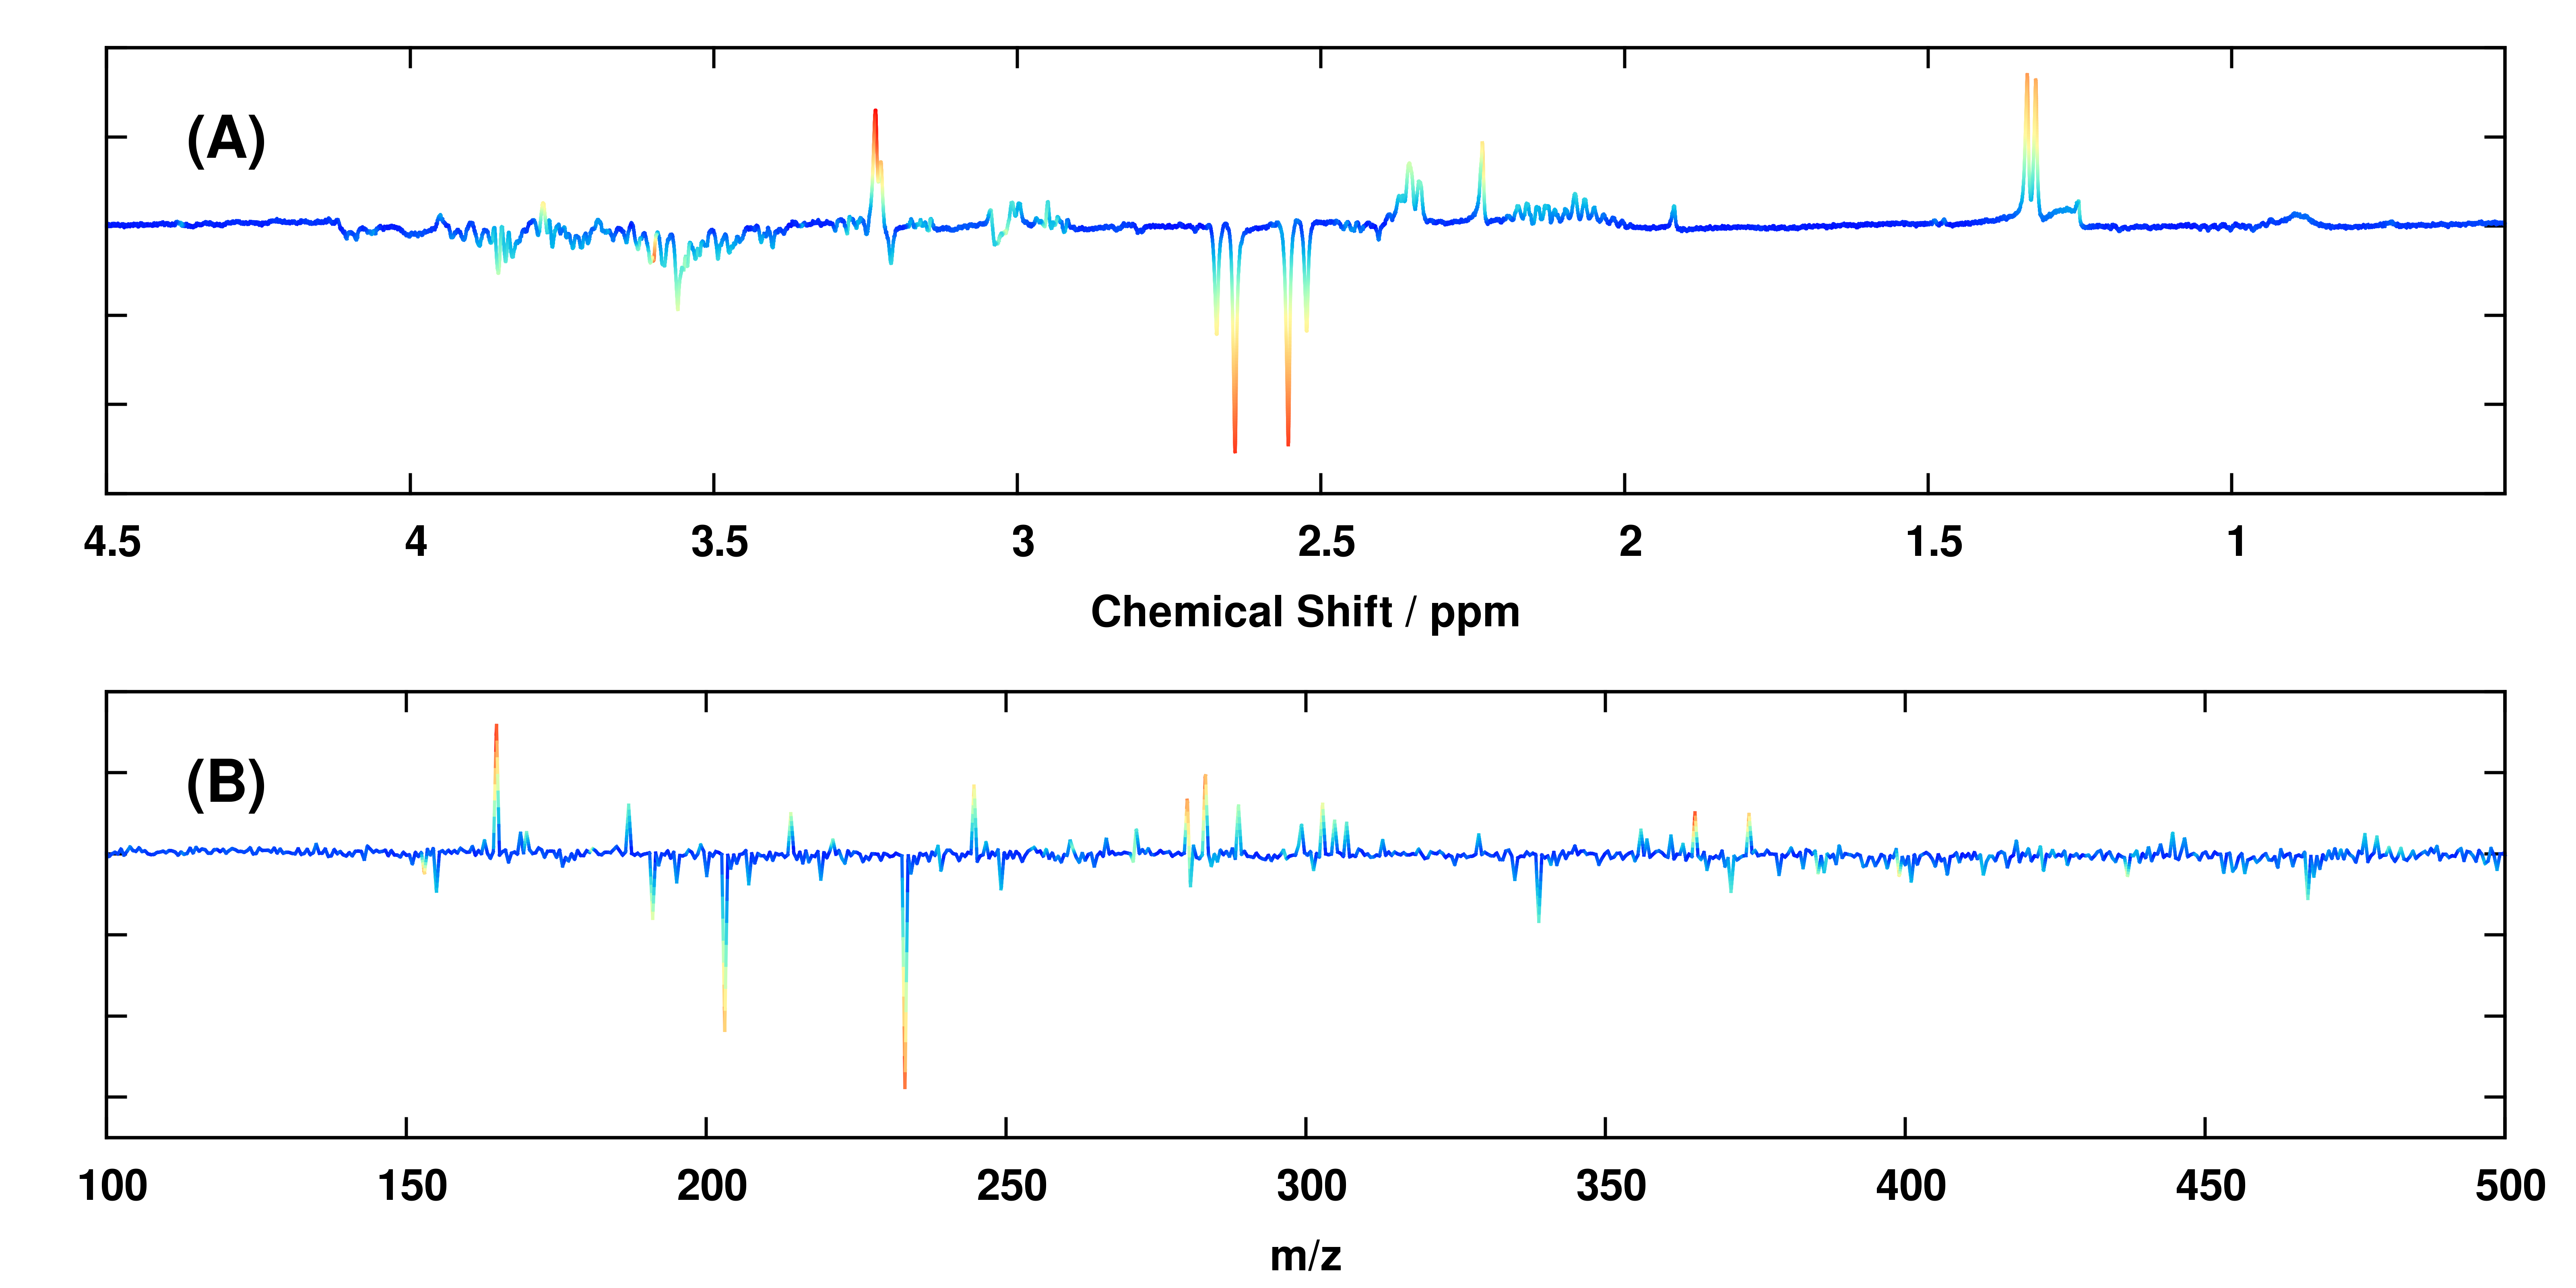
\includegraphics[width=6in]{figs/apps/13-mbopls-po.png}
\caption
      [Backscaled NMR and MS Orthogonal Block Loadings.]{
  {\bf Backscaled NMR and MS Orthogonal Block Loadings.}
  \\
  Backscaled orthogonal ({\bf A}) \hnmr{} NMR block and ({\bf B}) DI-ESI-MS
  block loadings from MB-OPLS-DA.
}
\label{figure.4.13}
\end{figure}

\begin{doublespace}
MB-PLS of the data yielded similar improvements in model information content.
Two significant components were identified
($R^2_Y = 0.9876, Q^2 = 0.9014 \pm 0.0185$) that clearly separated control and
paraquat treatment classes from all other classes in scores space
(\figref{4.10}{Figure 4.10}). CV-ANOVA testing produced a $p$ value
of $3.4 \times 10^{-4}$ and response permutation testing yielded
$p < 0.001$, indicating a reliable MB-PLS-DA model. Backscaled
first-component MB-PLS-DA loadings are shown in \figref{4.11}{Figure 4.11}.
Modeling the multiblock data with MB-OPLS and MCCV produced a
single predictive component and a single orthogonal component
($R^2_Y = 0.9031, Q^2 = 0.7084 \pm 0.0241$), making later interpretation
markedly simpler (cf. \figref{4.12}{Figures 4.12} and \figref{4.13}{4.13}).
Examination of cross-validated MB-OPLS-DA scores
(\figref{4.14}{Figure 4.14}) provides an excellent example of how PLS mixes
predictive and compensatory variation. In MB-OPLS super-scores, paraquat
treatment is distinctly separated from other neurotoxin treatment classes along
the orthogonal component ($\mathbf{t_o}$). In the MB-PLS model, this
distinction between paraquat and other drug treatments becomes mixed with the
variation that separates the control class from all drug treatments. However,
the two effects have been disentagled in the MB-OPLS model, providing richer
information about the differing mechanisms of each neurotoxic drug. Additional
orthogonal components would serve to further disentangle the two effects, at
the slight expense of model reliability. Validation of the MB-OPLS model by
CV-ANOVA resulted in a $p$ value equal to $5.5 \times 10^{-6}$, and permutation
testing corroborated CV-ANOVA with $p < 0.001$, once again indicating a
reliable supervised model.
\end{doublespace}

\begin{SCfigure}
\includegraphics[width=3.25in]{figs/apps/14-mbopls-t.png}
\caption
      [MB-OPLS-DA Cross-validated Scores.]{
  {\bf MB-OPLS-DA Cross-validated Scores.}
  \\
  Cross-validated scores generated from MB-OPLS-DA of the joint \hnmr{} NMR
  and DI-ESI-MS data. The OPLS filter within MB-OPLS has effectively rotated
  the super-scores of the MB-PLS model (Figure 4.10C) to better differentiate
  between class-predictive and class-orthogonal variation.
}
\label{figure.4.14}
\end{SCfigure}

\subsection{Conclusions}

\begin{doublespace}
The use of multiblock bilinear factorizations that capitalize on the
availability of blocking information afforded greater model interpretability
with the NMR and MS data than what was provided by single-block methods. The
neurotoxins dataset provided an opportunity to compare the results of LOOCV
and MCCV for optimal principal component count determination when marginally
predictive data is being modeled. As expected, MCCV was a less optimistic
estimator of model reliability than LOOCV, and produced more parsimonious PCA
decompositions. Finally, the dataset was an ideal proving ground for the new
MB-OPLS algorithm, as MB-PLS-DA had clearly mixed class-predictive variation
into multiple components. The use of MB-OPLS-DA resulted in more easily
interpretable backscaled loadings, and provided more information relating to
separations between control and drug treatment \emph{and} separations between
paraquat and other drug treatments (\figref{4.13}{Figure 4.13}).
\end{doublespace}

\section{Monte Carlo Analysis of Scores-space Separations}

\begin{doublespace}
While the necessity of validating PLS and OPLS models is well understood
within the statistics and chemometrics communities, it is an unfortunate fact
that validation of PLS and OPLS models is still infrequent in work published
by non-statistically oriented research groups \cite{brereton:jchemo2014b}.
This is especially true in the rapidly growing field of metabolomics, where
these methods are quite often -- and quite mistakenly -- considered surrogates
for PCA. PCA, PLS and OPLS are distinct modeling frameworks that achieve very
different goals (cf. \hyperlink{section.3.5}{Section 3.5}) and extract
different information from a dataset. However, the optimistically forced
class separations provided by PLS-DA and OPLS-DA have spawned a pattern of
misuse in metabolomics and related fields. When PCA fails to identify
significant separation between classes, untrained analysts may move to
biased, insufficiently vetted OPLS-DA models without considering the
statistical implications \cite{aksenov:anchem2014,mclaughlin:anchem2014}.
While it is certainly possible for OPLS-DA to identify separation when PCA
does not, the statistical significance of the separation must be validated
before conclusions are drawn from the results. Studies that lack proper
validation are automatically suspect from a statistical viewpoint, implying
that future attempts to reproduce their results may fail. Thus, validation
of all supervised models is an absolute requirement in chemometrics.
\\\\
Even before supervised models are trained, the separations between classes in
PCA scores space may be used as an informative qualitative predictor of
whether reliable OPLS-DA models may be trained on the same data. This section
presents practical guidelines on what level of OPLS-DA model reliability may
be expected based solely on PCA class separations.
\end{doublespace}

\subsection{Materials and Methods}

\begin{doublespace}
A Monte Carlo simulation was performed using MVAPACK \cite{worley:acscb2014}
to analyze the relationship between class separations in PCA scores space and
OPLS-DA cross-validation metrics, as a function of spectral noise content.
Two data matrices that both contained highly significant class-discriminating
variation were used within two parallel simulations.
\end{doublespace}

\subsubsection{Initial Datasets}

\begin{doublespace}
Two classes of observations (Light and Medium Decaffeinated) from the binned
data matrix were extracted from the latest version of the Coffees
dataset \cite{worley:acscb2014}. The resulting data matrix (referred to as
$\mathbf{X}$: $N = 32, K = 284$) contains a highly significant separation
between the two classes based on caffeine 1D \hnmr{} NMR spectral features.
A second dataset, generated from a comparison of two chemically defined cell
growth media, was used to provide further support for the trends observed
during Monte Carlo analysis of the Coffees data matrix. The resulting Media
data matrix ($N = 50, K = 238$) also contains highly significant separation
between two classes based on 1D \hnmr{} NMR spectral features.
\\\\
Prior to Monte Carlo simulation, the $\ell_2$ norm (largest singular value) of
each data matrix $\mathbf{X}$ was computed and stored as $\sigma_{max}$. A set
of 50 noise standard deviations ($\sigma$) where each value ranged from
$\sigma_{max}/500$ to $\sigma_{max}/10$. For each noise standard deviation,
a set of 200 Monte Carlo iterations was performed. Another set of 200
iterations was also performed on each original data matrix $\mathbf{X}$ without
any added noise.
\end{doublespace}

\subsubsection{Monte Carlo Simulation}

\begin{doublespace}
At each Monte Carlo iteration, an $N \times K$ real matrix of noise values was
drawn as $NK$ independently and identically distributed samples from a
zero-mean normal distribution having a standard deviation of $\sigma$,
corresponding to the current noise value as described above. The data matrix
$\mathbf{X}$ was summed with the noise matrix, and a three-component ($A = 3$)
PCA model was computed on the resulting sum ($\mathbf{X'}$) after unit variance
scaling \cite{vandenberg:bmcg2006} using a NIPALS algorithm
\cite{jolliffe2002}. The explained variation (\rsq{}) of each principal
component was computed as described in \hyperlink{section.3.6}{Section 3.6}.
A Monte Carlo leave-$n$-out cross-validation (MCCV) was performed based on the
modified method of Krzanowski and Eastment \cite{eshghi:cils2014} in order to
obtain a per-component predictive ability (\qsq{}) statistic. A seven-fold
partitioning of observations and variables, randomly resampled ten times, was
performed for each PCA MCCV run. Following PCA model training, the Mahalanobis
distance between the two classes was computed using PCA scores
\cite{demaesschalck:cils2000}.
\\\\
After computation of the Mahalanobis distance, the noisy data matrix
$\mathbf{X'}$ was Pareto-scaled and subjected to OPLS-DA using a Pareto-scaled
binary $(0,1)$ response vector ($\mathbf{y}$) and a NIPALS OPLS algorithm
\cite{trygg:jchemo2002}. A one-component ($A_p = 1, A_o = 1$) OPLS model was
constructed, from which backscaled predictive loadings were extracted by
dividing by the coefficients obtained from Pareto scaling
\cite{cloarec:anchem2005b}. The Pearson correlation coefficient between
backscaled loadings and the known ``true'' loadings --
$\mathrm{corr}(\mathbf{p},\mathbf{p_0})$ -- was computed for later
visualization. Explained variation (\rsqy{}) was computed as described in
\hyperlink{section.3.6}{Section 3.6}. A Monte Carlo leave-$n$-out internal
cross-validation of the OPLS model was performed using a seven-fold
partitioning of the data matrix that was randomly resampled ten times
\cite{xu:cils2001}. Predictive ability (\dqsq{}) statistics were computed as
the mean \dqsq{} obtained from MCCV results \cite{westerhuis:metab2008b}.
Thus, each OPLS model contained a set of ten fitted residual matrices from
cross-validation available for use in CV-ANOVA significance testing
\cite{eriksson:jchemo2008}. During CV-ANOVA calculations, the median values
of mean square error (MSE) were computed from all residual matrices, and the
ratio of median fitted MSE to median residual MSE was calculated to yield an
$F$-statistic for $p$ value generation.
\end{doublespace}

\begin{figure}[ht!]
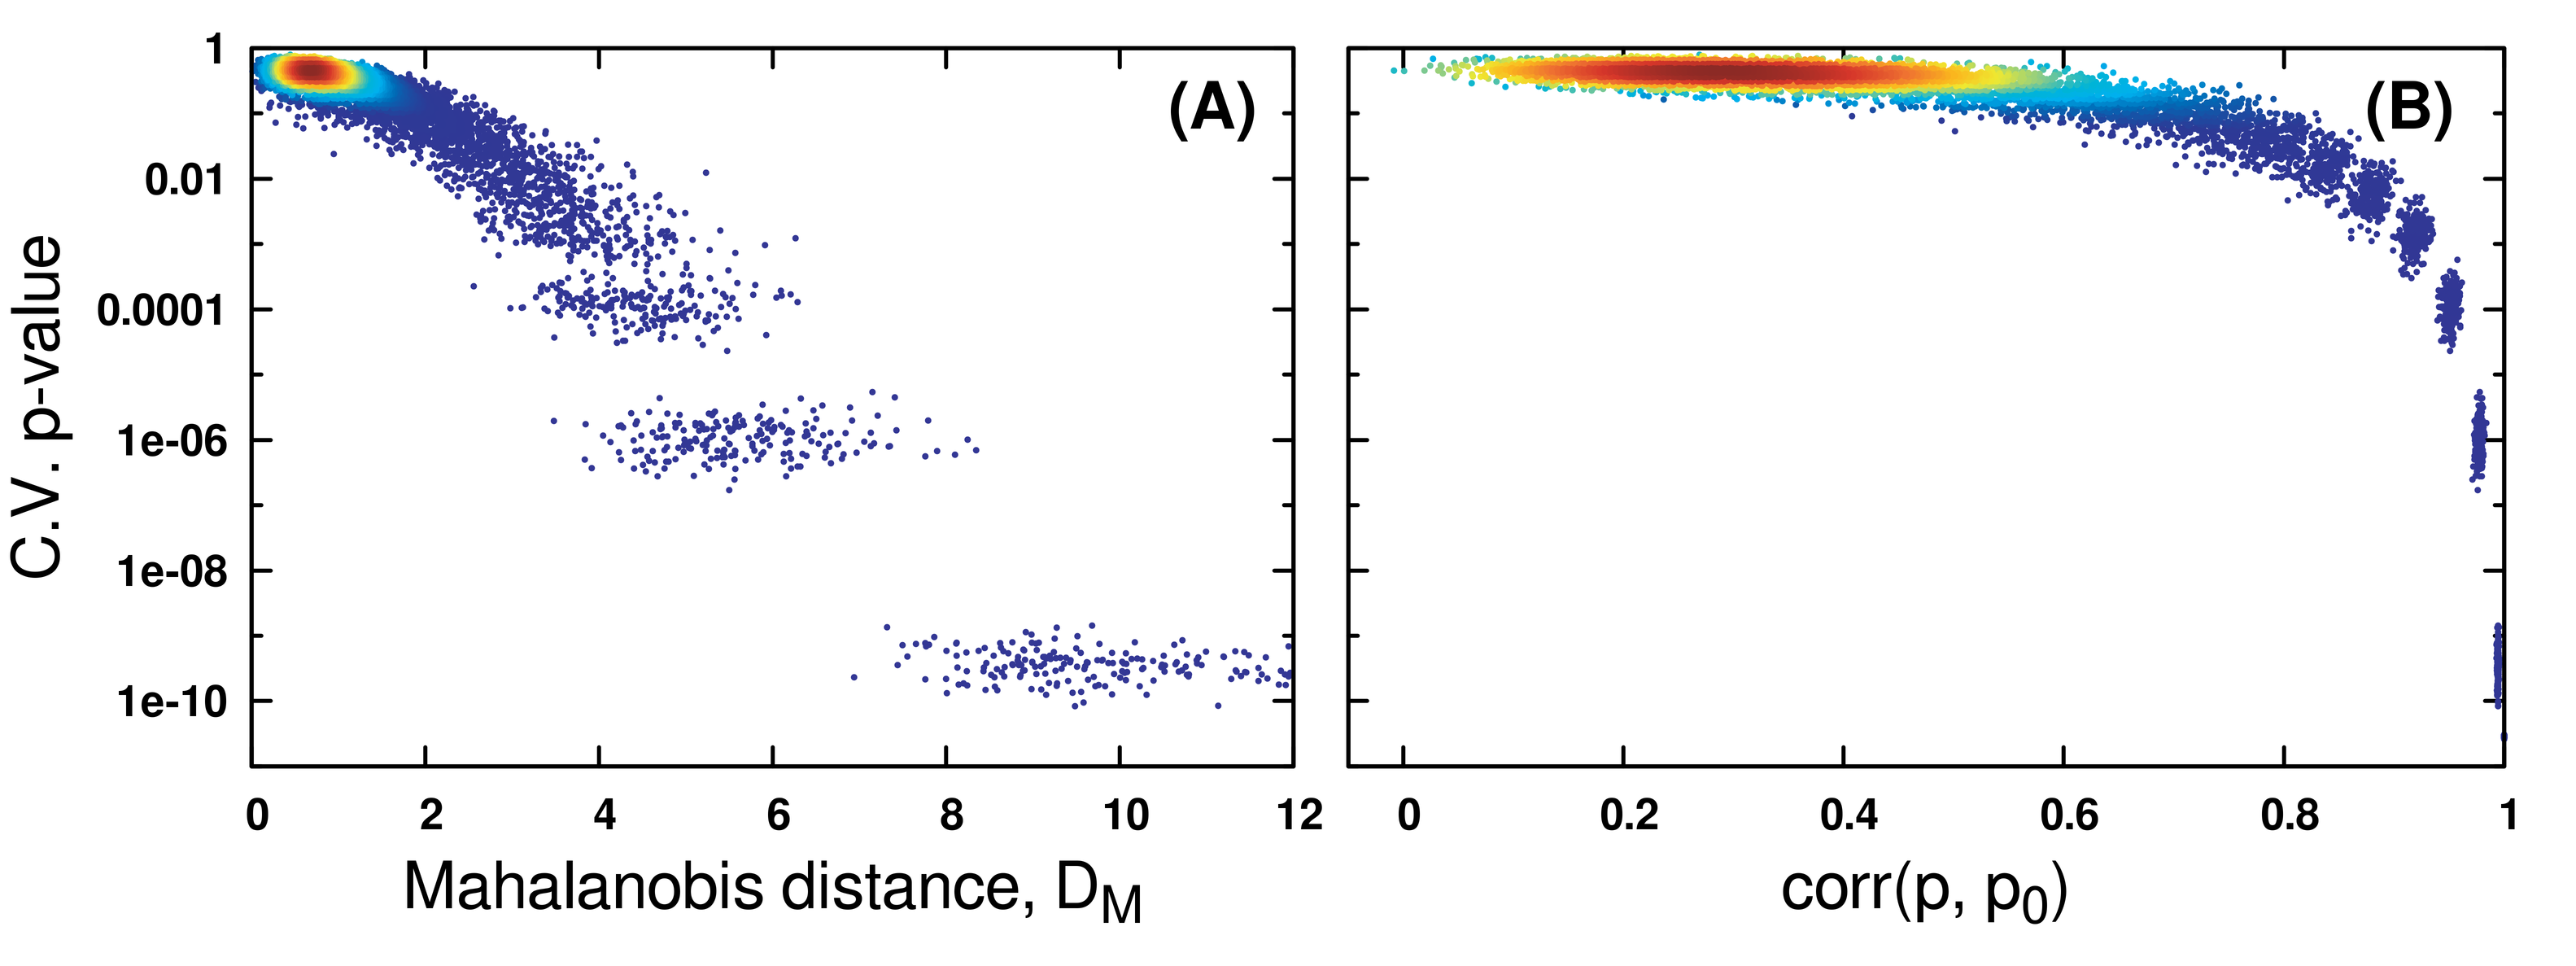
\includegraphics[width=6in]{figs/apps/15-scatter-a.png}
\caption
      [Monte Carlo Results for the Coffees Data Matrix.]{
  {\bf Monte Carlo Results for the Coffees Data Matrix.}
  \\
  Relationships to OPLS-DA CV-ANOVA $p$ values obtained through Monte Carlo
  simulation of ({\bf A}) the Mahalanobis distance ($D_M$) between classes
  in PCA scores space, and ({\bf B}) the correlation between OPLS-DA model
  predictive loadings given noisy data ($\mathbf{p}$) and loadings obtained
  on the original Coffees data matrix ($\mathbf{p_0}$). The density of points
  in both panels is indicated by coloring, where red indicates high point
  density and blue indicates low density.
}
\label{figure.4.15}
\end{figure}

\begin{figure}[ht!]
\includegraphics[width=6in]{figs/apps/16-scatter-b.png}
\caption
      [Monte Carlo Results for the Media Data Matrix.]{
  {\bf Monte Carlo Results for the Media Data Matrix.}
  \\
  Summarization of Monte Carlo results from the Media data matrix. See Figure
  4.15 for more details.
}
\label{figure.4.16}
\end{figure}

\subsection{Results and Discussion}

\begin{doublespace}
As expected, PCA scores-space class separations rapidly decreased as noise
was added to the data. Addition of noise also forced a rise in OPLS-DA
cross-validation statistics. As a result, a strong exponential relationship
is observed between Mahalanobis distances calculated from PCA scores and
CV-ANOVA $p$ values from OPLS-DA models (\figref{4.15}{Figures 4.15A} and
\figref{4.16}{4.16A}). Because PCA modeling uses no class membership
information, the scores-space distances in these figures are essentially the
least biased method of appraising discrimination ability. As the two classes
become less distinguishable based on their spectral measurements, PCA will
expose less separation between their scores. When PCA fails to expose class
separation, OPLS-DA will continue to do so
\emph{at the expense of model reliability}, as it is relying on weaker
sources of variation in the noisier data. While the exact form of the
relationship between distance and $p$ value will depend on the input data and
responses, this analysis provides clear evidence that distances between classes
in PCA scores may be used as a qualitative ruler of future supervised model
reliability.
\end{doublespace}

\begin{figure}[ht!]
\includegraphics[width=6in]{figs/apps/17-lines.png}
\caption
      [Effect of Noise on Loadings and CV-ANOVA Statistics.]{
  {\bf Effect of Noise on Loadings and CV-ANOVA Statistics.}
  \\
  ({\bf A}) Decrease of correlation between estimated loadings ($\mathbf{p}$)
  and true loadings ($\mathbf{p_0}$) as varying degrees of noise are added to
  the Coffees (red) and Media (blue) data matrices. Light shaded regions
  indicate confidence intervals of plus or minus one standard deviation from
  the mean correlation. A value of 1x additive noise corresponds to a noise
  standard deviation equaling 0.002 times the data matrix $\ell_2$ norm.
  ({\bf B}) Increase of $p$ values from CV-ANOVA validation as varying degrees
  of noise are added to the data matrices. Shaded regions indicate plus or
  minus one standard deviation from the median $p$ value.
}
\label{figure.4.17}
\end{figure}

\begin{doublespace}
The shrinkage of Mahalanobis distances as data matrix noise increases occurs
concomitantly with a rapid loss of correlation between ideal OPLS predictive
loadings and estimated loadings (\figref{4.15}{Figures 4.15B},
\figref{4.16}{4.16B} and \figref{4.17}{4.17A}). It is critical to note that
class separations in OPLS scores space do not appreciably decrease
(\figref{4.18}{Figure 4.18}) with the decreased loading correlations.
In effect, the OPLS model has identified different, \emph{less reliable}
sources of variation in the noisy data matrix in order to maintain class
separation. OPLS-DA requires only that some variation in the measured data
correlates with class membership, regardless of whether that variation is
signal or noise \cite{wold:cils2001,trygg:jchemo2002,gottfries:jchemo2008}.
When the true predictive spectral features that reflect the underlying
biochemistry have become masked by noise, OPLS-DA will shift its focus to the
variation that best predicts class membership. Because OPLS-DA provides the
most optimistic result possible, validation becomes a necessity.
\end{doublespace}

\begin{figure}[ht!]
\begin{center}
  \includegraphics[width=5in]{figs/apps/18-scores.png}
\end{center}
\caption
      [Effect of Noise on PCA and OPLS-DA Scores.]{
  {\bf Effect of Noise on PCA and OPLS-DA Scores.}
  \\
  Comparison of representative PCA ({\bf A}, {\bf C}, {\bf E}) and OPLS-DA
  ({\bf B}, {\bf D}, {\bf F}) scores resulting from modeling the original
  data matrix ({\bf A}, {\bf B}), the 4x noisy data matrix ({\bf C}, {\bf D}),
  and the 20x noisy data matrix ({\bf E}, {\bf F}). Ellipses represent
  the 95\% confidence regions for class membership.
}
\label{figure.4.18}
\end{figure}

\begin{doublespace}
These Monte Carlo simulations once again illustrate how noise can masquerade
as class-predictive variation in statistical analyses of high-dimensional
spectral measurements. Moreover, the simulations touch on an often-overlooked
distinction between class separations and
\emph{reliable, statistically significant} class separations in PCA/PLS scores
space. Although PLS and OPLS may separate classes in situations where PCA
cannot, this outcome should raise a red flag to the analyst that the model
is suspect and the data may not sufficiently predict class membership. Only
after rigorous cross-validation can it be safely inferred that OPLS-DA class
separations are reliable and significant. If cross-validated estimates of
OPLS-DA scores still separate the desired classes, and CV-ANOVA and permutation
testing report significant $p$ values, the models may be used for chemical
inference. If cross-validation is left unreported, conclusions drawn from the
models must be met with strong skepticism \cite{westerhuis:metab2008a,
  brereton:jchemo2014b}.
\\\\
The results of these Monte Carlo analyses relating PCA scores-space separations
to OPLS-DA cross-validation metrics effectively summarize the reasons why
rigorous cross-validation is necessary in chemometric studies relying on
multivariate methods. More specifically, they reaffirm the importance of PCA
as a first-pass unsupervised tool in metabolic fingerprinting and untargeted
metabolic profiling studies, where class separations in scores space are often
the sole basis for further experimentation. It is an unfortunate common
practice in such studies to dismiss completely overlapped classes in PCA scores
space and move ahead to (usually un-validated) supervised methods such as PLS
and OPLS that force scores-space separation. Such practices almost guarantee
the irreproducibility of any conclusions drawn from trained multivariate
models, as the relationship from Monte Carlo simulation indicates. It is
therefore highly recommended that methods which assign Mahalanobis
distance-based confidence ellipses to classes in PCA scores
\cite{worley:abio2013}, report cross-validation estimated scores plots for
PLS and OPLS models \cite{westerhuis:metab2008a}, and provide one or more
cross-validated metrics during model training \cite{worley:acscb2014} be used
in these studies whenever possible.
\\\\
These analyses are only a case study for two specific data matrices, and are
not meant to provide a quantitative relationship between any of the discussed
metrics over all possible metabolomics studies. Instead, they lend positive
numerical support to the recommendations that analysts rigorously validate
their models by multiple means, including CV-ANOVA, response permutation
testing, and even qualitative examination of PCA scores-space class
separations. It is hoped that this work may be used to further promote
best practices of supervised multivariate model training and validation in
the community.
\end{doublespace}

\bibliographystyle{abbrv}
\bibliography{bworley}

